\chapter{Výsledky detekce novosti algoritmem Extreme Seeking Entropy}\label{chap:vysledky}
V dalším textu jsou shrnuty výsledky algoritmu Extreme Seeking Entropy kterých bylo v rámci práce na dizertační práci dosaženo. Výsledky použití ESE pro detekci pertubace v chaotické časové řadě Mackey-Glass je uvedena v podkapitole \ref{chap:mdpi_mg}. Dále jsou uvedeny výsledky pro: detekci změny rozptylu šumu v náhodném datovém toku (viz podkapitola \ref{chap:mdpi_noise_change}, detekci skokové změny parametrů generátoru signálu (viz podkapitola \ref{chap:mdpi_stepchange}), detekci náhle absence šumu (viz podkapitola \ref{chap:mdpi_noise_ext}), detekci změny trendu (viz podkapitola \ref{chap:mdpi_trendchange} a detekci epilepsie v záznamu myšího EEG (viz podkapitola \ref{chap:mdpi_eeg}). Dále jsou uvedeny výsledky vyhodnocení úspěšnosti detekce skokové změny parametrů generátoru signálu (viz podkapitola \ref{chap:mdpi_step_stats}) a úspěšnosti detekce skokové změny trendu (viz podkapitola \ref{chap:mdpi_trendchange_evaluation}). V posledních dvou kapitolách je potom vyhodnocení ROC křivky (receiver operating characteristic) pro detekci změny trendu (viz podkapitola \ref{chap:appel_roc}) a experimentální vyhodnocení výpočetní náročnosti metod odhadu parametrů zobecněného Paretova rozdělení (viz podkapitola \ref{chap:appel_gpd}).
\par Výsledky v podkapitolách \ref{chap:mdpi_mg}-\ref{chap:mdpi_trendchange_evaluation} byly publikovány v \cite{ese_mdpi}. Výsledky v podkapitolách \ref{chap:appel_roc} a \ref{chap:appel_gpd} pak v publikacích \cite{appel2,appel3}.

\section{Chaotická časová řada Mackey-Glass a detekce pertubace}\label{chap:mdpi_mg}
Tento experiment byl proveden pro porovnání s výsledky uvedenými v publikaci \cite{ivoLE1}, která je první publikací o algoritmu LE (viz kapitola \ref{chap:LE}). Experiment spočívá v detekci pertubovaného vzorku v chaotické časové řadě, která je výsledkem řešení Mackey-Glassovy rovnice \cite{mackey}.
\begin{equation}
    \frac{dy(t)}{dt}= \beta \cdot \frac{ y(t-\tau)}{1 + y^\alpha(t-\tau)} - \gamma y(t)
\end{equation}
přičemž parametry $\alpha = 10$, $\beta = 0.2$, $\gamma = 0.1$ and $\tau = 17$ byly vybrány tak, aby řešením této rovnice byla chaotická časová řada. Celkem bylo vygenerováno 701 vzorků. Data v diskrétní časový okamžiku $k=523$ pak byly pertubovány podle následujícího předpisu.
\begin{equation}
    y(523) = y(523) + 0.05 \cdot y(523)
\end{equation}
Výsledná časová řada a detail pertubace je znázorněn na obrázku \ref{fig:mackey_details}. Jako adaptivní filtr byl zvolen QNU (resp. Volterrův filtr) jehož vstupem jsou 4 časově spožděné hodnoty časové řady $y(k-1)$, $y(k-2)$, $y(k-3)$, $y(k-4)$. Hodnoty adaptivních vah tohoto filtru byly adaptovány algoritmem NLMS. Struktura filtru byla zvolena stejně jako v \cite{ivoLE1}. Rychlost učení během experimentu byla nastavena na $\mu=1$. Metoda POT byla zvolena podle rovnice \ref{eq:l1} a délka okna pro detekci novosti algoritmem ESE byla nastavena na $n_s=300$. 
\par 
Výstup adaptivního filtru a chyba predikce jsou znázorněny na obrázku \ref{fig:mackey_results}. Výsledky metod detekce novosti jsou zobrazeny na obrázku \ref{fig:mackey_results_nd}. Z obrázku je patrné, že globální maximum průběhu $ESE$ odpovídá pertubovaným datům. Globální maximum metod $ELBND$ a $LE$ odpovídá vzorku u něhož byla největší chyba predikce. Hodnoty prahů algoritmu LE byly zvoleny $\boldsymbol{\alpha}=\{4,5,6,7,8,9\}$ a délka okna byla nastavena na $m=30$.


\begin{figure}[!ht]
    \centering
    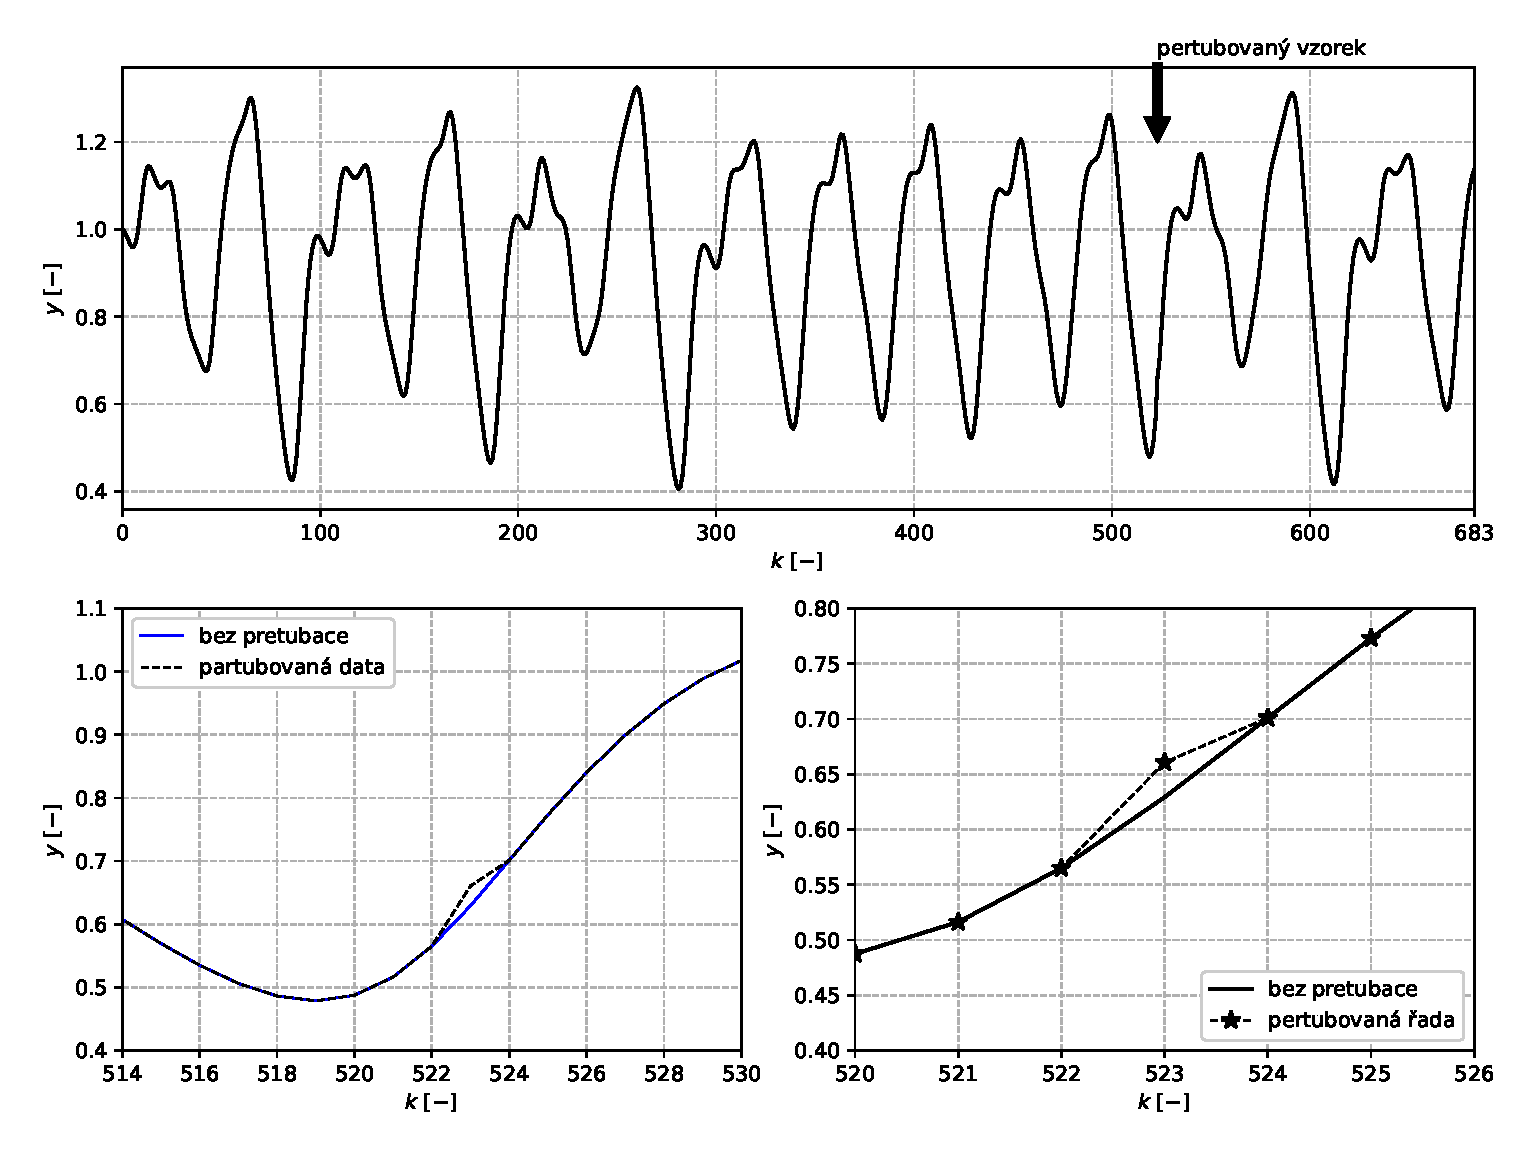
\includegraphics[scale=0.56]{IMG/mdpi/mackeydetails_diz.eps}
    \caption{Horní graf zobrazuje celou datovou řadu. Spodní grafy zobrazují detail pertubovaného vzorku v diskrétní časový okamžik $k=523$.}
    \label{fig:mackey_details}
\end{figure}
\begin{figure}[!ht]
    \centering
    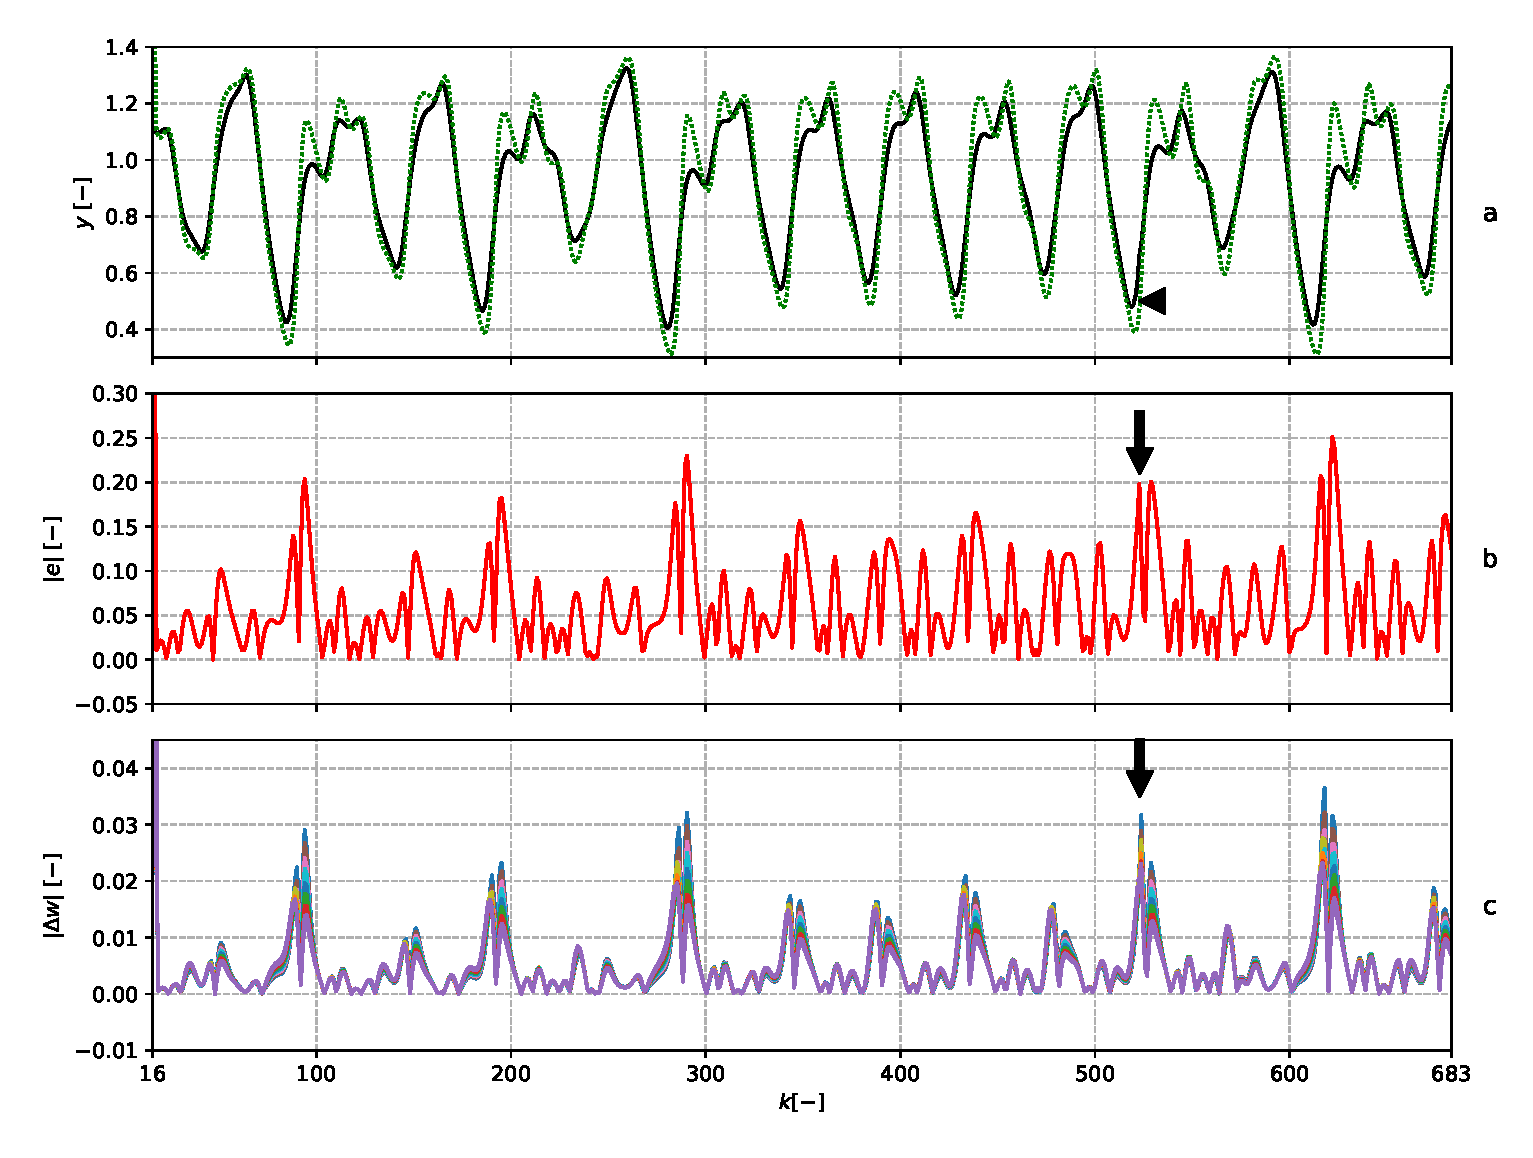
\includegraphics[scale=0.56]{IMG/mdpi/mackey_results.eps}
    \caption{Graf (a) zobrazuje datovou řadu s pertubací (černá plná čára) a výstup adaptivního filtru (tečkovaná zelená čára). Pertubovaný vzorek je označen černou šipkou. Graf (b) zobrazuje velikost chyby predikce $e$ (resp. její absolutní hodnotu). Na grafu (c) jsou znázorněny přírůstky adaptivních vah filtru (resp. absolutní hodnotu těchto přírůstků).}
    \label{fig:mackey_results}
\end{figure}

\begin{figure}[!ht]
    \centering
    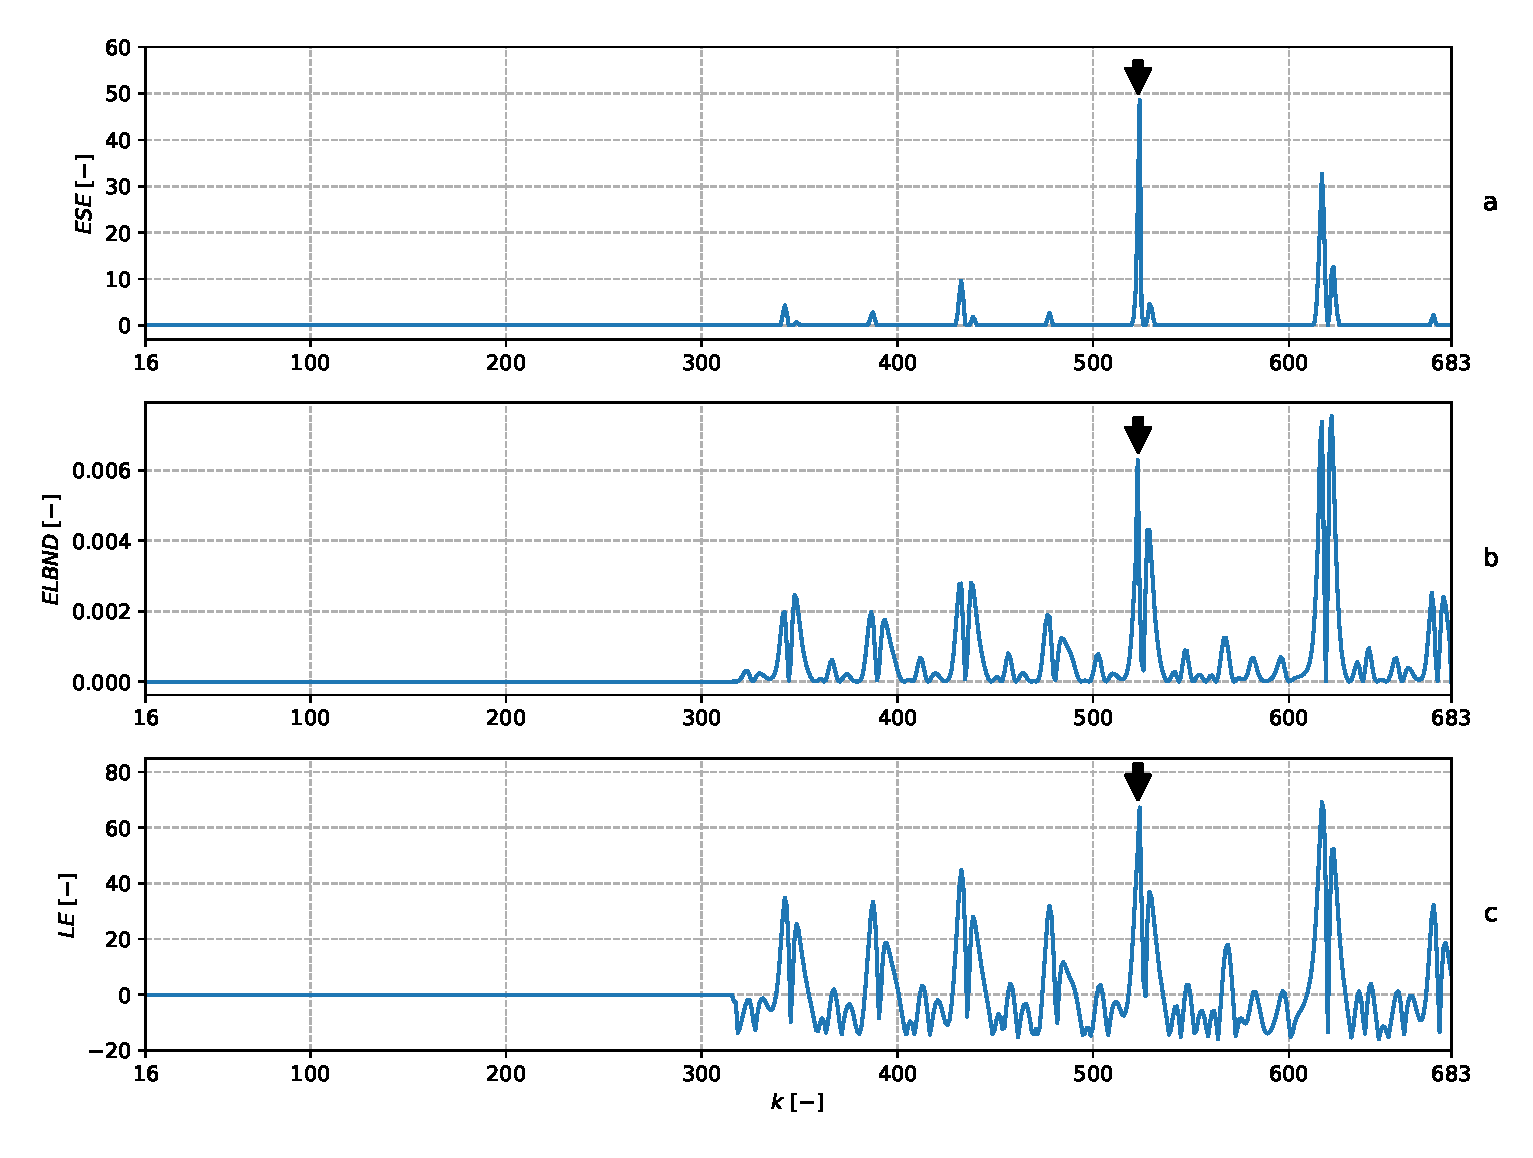
\includegraphics[scale=0.57]{IMG/mdpi/mackey_results_nd.eps}
    \caption{Graf (a) zobrazuje hodnotu ESE. Prvních 300 vzorků je hodnota ESE nulová, protože délka okna pro vyhodnocování novosti $n_s=300$. Graf (b) zobrazuje výsledky algoritmu ELBND. Prvních 300 výsledků ELBND je pro názornost vynecháno. Graf (c) zobrazuje výsledky algoritmu LE.}
    \label{fig:mackey_results_nd}
\end{figure}

\section{Detekce změny rozptylu šumu v náhodném datovém toku}\label{chap:mdpi_noise_change}
Tato případová studie je navržená na základě problému, který se vyskytuje v použití hybridních navigačních systémů využívajících GPS (Global Positioning System) senzory pro navigaci výpočtem \cite{dead}. Smyslem experimentu je demonstrovat možnost využití algoritmu ESE pro detekci změn rozptylu šumu v náhodných datech.
\par
Uvažujme dva vstupy $x_1(k)$ a $x_2(k)$ a výstup generátoru signálu $y(k)$ takový, že
\begin{equation}
y(k)=x_1(k)+x_2(k)+x_1(k)\cdot x_2(k)+v(k)
\end{equation}
kde člen $v(k)$ reprezentuje aditivní Gaussovský šum který je přidán k výstupu generátoru $y(k)$. Přidaný šum má nulovou střední hodnotu a směrodatnou odchylku $\sigma_n=0.1$, takže $v(k)\sim N(0,1)$. Hodnoty vstupů jsou v každém diskrétním časovém okamžiku vybrány náhodně z rovnoměrného rozdělení na intervalu $\langle 0,\rangle$. V diskrétním časovém okamžiku $k=500$ dojde ke změně směrodatné odchylky šumu na hodnota $\sigma_n=0.2$, $v(k) \sim N(0,0.2)$. Adaptivní filtr v tomto experimentu byl QNU ve tvaru
\begin{equation}
\hat{y}(k)=w_1\cdot x_1(k) + w_2\cdot x_2(k)+w_3\cdot x_1(k)\cdot x_2(k)
\end{equation}
tak,  že jeho struktura odpovídá struktuře generátoru signálu. Adaptivní parametry filtru byly adaptovány algoritmem GNGD. Rychlost učení byla nastavená jako $\mu=1$. Metoda POT byla zvolena podle rovnice \ref{eq:l2} a délka okna $n_s=500$. Výsledky experimentu jsou zobrazeny na obrázku \ref{fig:noise_changed}. Apriorní hodnoty parametrů GPD byly stanoveny na základě 500 vzorků, které nejsou v následujícím obrázku \ref{fig:noise_changed} zobrazeny. Globální maximum ESE odpovídá změně směrodatné odchylky šumu $\sigma_n$. Detekce pomocí algoritmů LE a ELBND je o několik vzorků opožděná. Pro výpočet LE byl použit vztah \ref{eq:le_direct_padasip} a délka okna byla nastavena na $M=300$. Výpočet ELBND byl proveden podle rovnice \ref{eq:elbnd2}.

\begin{figure}[ht!] 
    \centering
    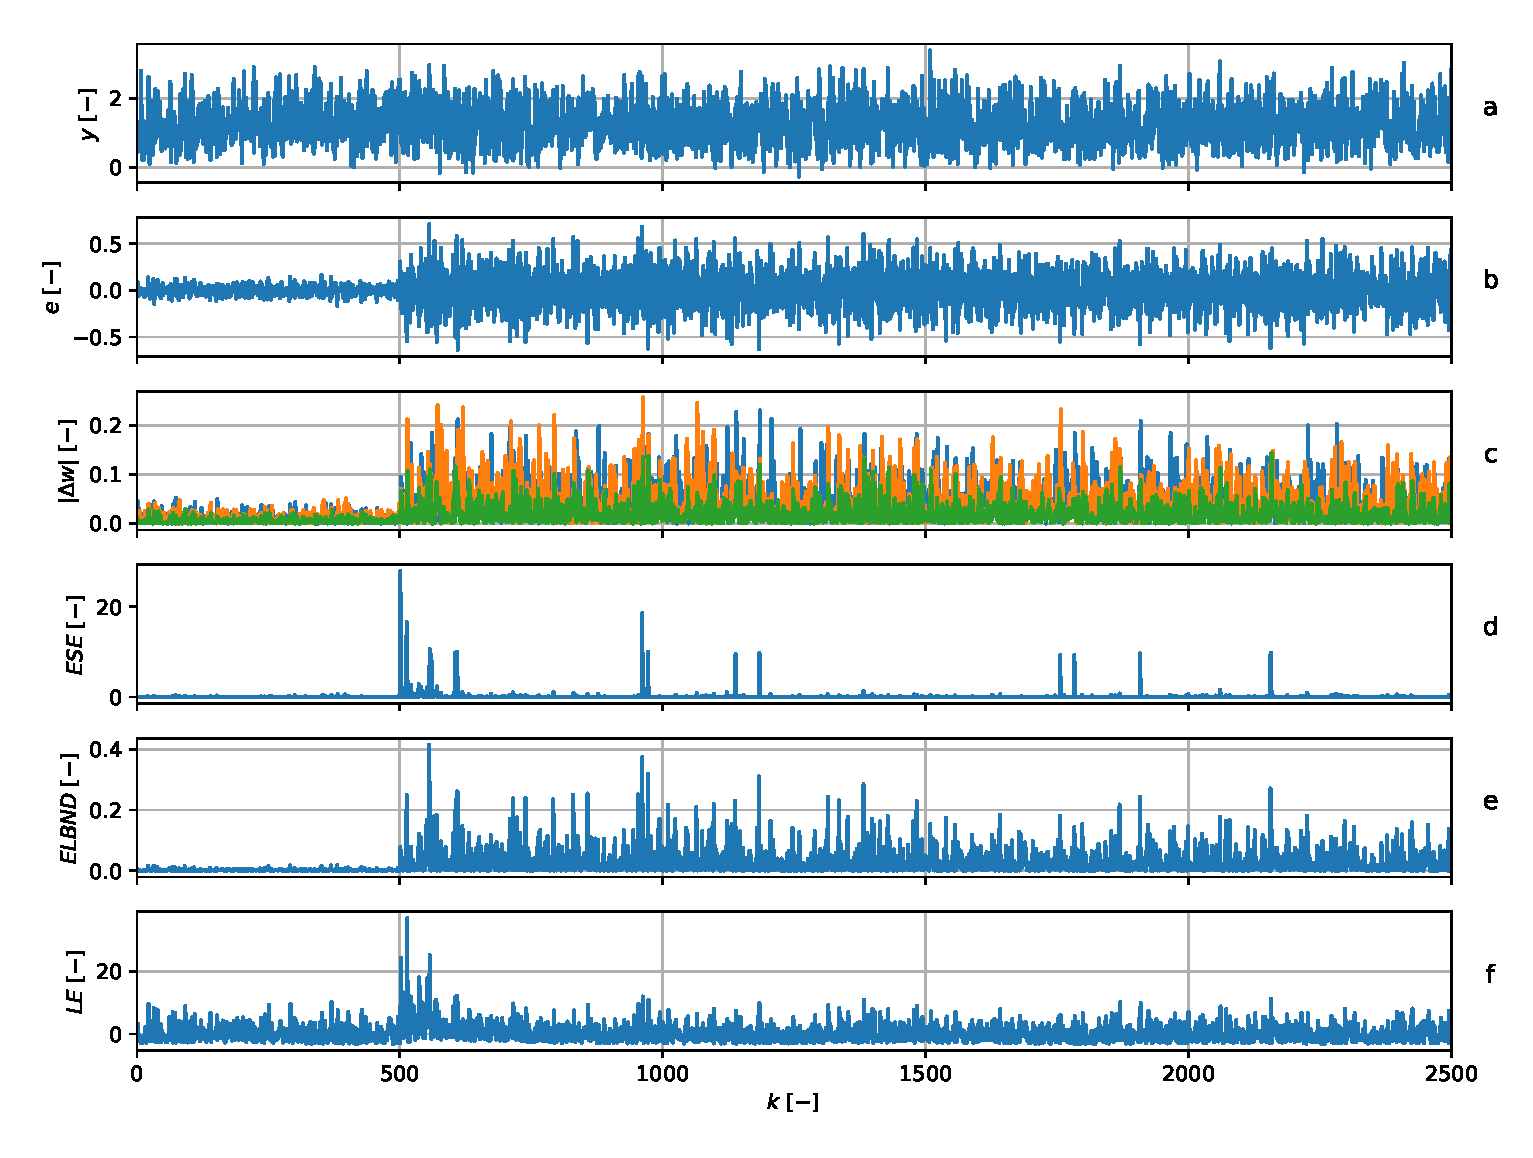
\includegraphics[scale=0.60]{IMG/mdpi/noise_change.eps}
    \caption{Detekce změny rozpylu šumu. Na grafu (a) jsou zobrazeny data z generátoru (modrá) a výstup z adaptivního filtru (zelená). Na grafu (b) je vynesena chyba filtru $e(k)$. Graf (c) zobrazuje velikosti přírůstků adaptivních parametrů filtru. Na grafu (d) jsou zobrazeny hodnoty ESE. V diskrétní časový okamžik $k=500$ je patrný značný nárůst v ESE, který reflektuje změnu směrodatné odchylky aditivního šumu. Na dalších grafech (e) a (f) jsou zobrazeny výsledné hodnoty algoritmů ELBND a LE.}
    \label{fig:noise_changed}
\end{figure}

\section{Detekce skokové změny parametrů generátoru signálu}\label{chap:mdpi_stepchange}
Tato případová studie je motivována problémem, který vzniká při sledování vícero náhodných datových toků \cite{stepchange} u kterých se kontroluje, zda nedošlo ke změně vlastností jejich generátoru. Uvažujme opět dva vstupy $x_1(k)$, $x_2(k)$ a výstup generátoru signálu ve tvaru
\begin{equation}
y(k)=x_1(k)+x_2(k)+x_1(k)\cdot x_2(k) + v(k)
\end{equation} 
kde člen $v(k)$ reprezentuje gaussovský aditivní šum s nulovou střední hodnotou a směrodatnou odchylkou $\sigma_n=0.1$, $v \sim N(0,0.1)$. Hodnoty vstupů $x_1(k)$ a $x_2(k)$ jsou v každém diskrétním časovém okamžiku náhodně vybrány z rovnoměrného rozdělení, $x_1(k) \sim U(0,1)$ resp. $x_2(k) \sim U(0,1)$. V časový diskrétní okamžik $k=500$ dojde ke změně parametrů generátoru, a výstup generátoru přejde do tvaru
\begin{equation}\label{eq:stepchange_dataset}
y(k)=0.4\cdot x_1(k) + 1.6x_2(k)+0.99x_1(k)\cdot x_2(k) + v(k).
\end{equation}
Jako adaptivní filtr byl v tomto případě zvolen QNU, jehož struktura odpovídá generátoru dat. Výstup tohoto filtru je tedy
\begin{equation}
\hat{y}(k)=w_1\cdot x_1(k)+w_2\cdot x_2(k)+w_3\cdot x_1(k)\cdot x_2(k)
\end{equation}
přičemž adaptivní parametry uvedeného filtru jsou adaptovány algoritmem GNGD. Rychlost učení během experimentu byla nastavena na $\mu=1$. POT metoda byla zvolena podle rovnice \ref{eq:l1} a parametr délky okna byl $n_s=500$. Apriorní hodnota parametrů GPD a dat pro LE byla získána použitím 500 vzorků dat (vygenerovaných podle rovnice \ref{eq:stepchange_dataset}). Výsledky experimentu jsou znázorněny na obrázku \ref{fig:step_change}. Z obrázku je patrné, že pomocí algoritmu ESE se podařilo detekovat skokovou změnu parametrů, čemuž odpovídá výrazné globální maximum v ESE. Globální maximum v LE neodpovídá skokové změně parametrů generátoru a detekce pomocí algoritmu ELBND je opožděná.

\begin{figure}[h!]
    \centering
    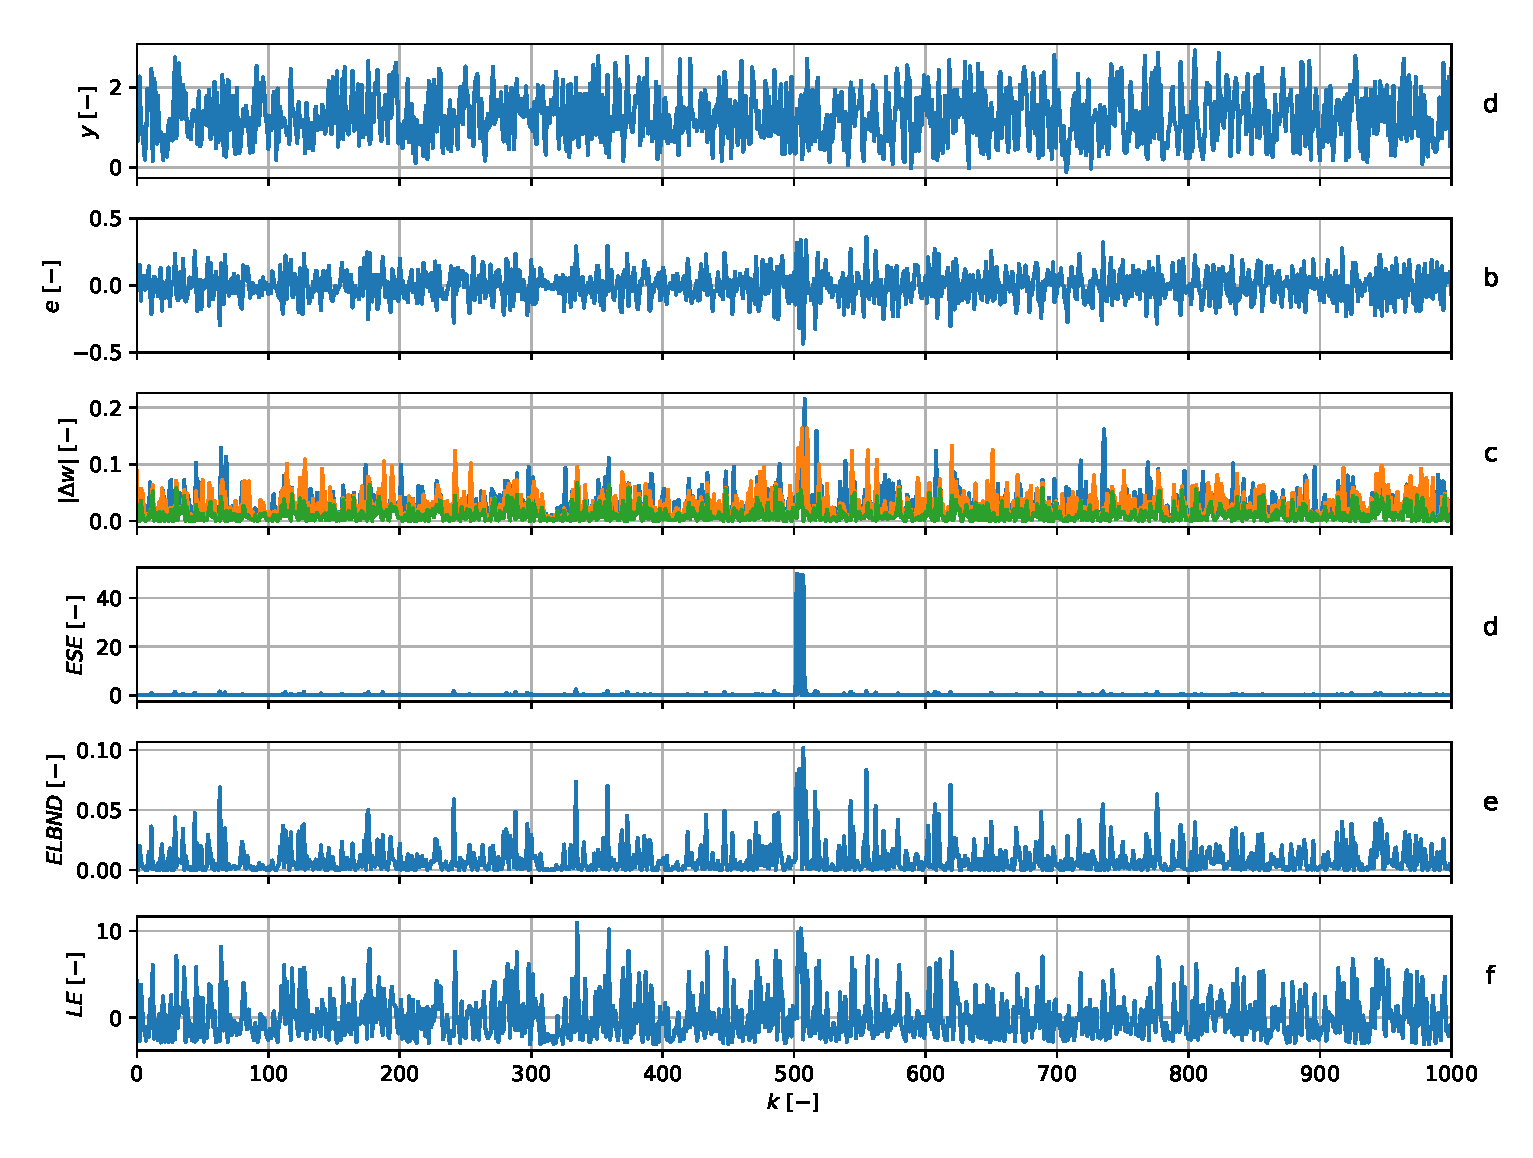
\includegraphics[scale=0.6]{IMG/mdpi/stepchange.eps}
    \caption{Detekce skokové změny generátoru signálu.Na grafu (a) je zobrazena původní časová řada (modrá). Graf (b) zobrazuje chybu filtru $e$. Na grafu (c) jsou zobrazeny velikosti přírůstků adaptivních vah filtru. Na grafu (d) jsou pak výsledky algoritmu ESE, přičemž k skokové změně parametrů generátoru signálu došlo v diskrétní časový okamžik $k=500$. Je tedy vidět globální maximum v ESE odpovídající úspěšné detekci. Na grafech (e) a (f) jsou pak výsledky metod ELBND a LE. Detekci algoritmem ELBND lze považovat za úspěšnou. Detekce algoritmem LE byla neúspěšná. Globální maximum LE je v diskrétním časovém okamžiku $k=338$, který neodpovídá skokové změně parametrů generátoru signálu.}
    \label{fig:step_change}
\end{figure}

\section{Detekce náhlé absence šumu}\label{chap:mdpi_noise_ext}
V této kapitole je ukázáno, že lehce modifikovaný algoritmus ESE může být využit také k detekci neobvykle malých změn parametrů adaptivního filtru. Oproti standardní variantě ESE budeme vyhodnocovat neobvykle malé přírůstky vah adaptivního filtru. Takže jediná změna v algoritmu je, že metodou POT budeme vybírat pouze nejmenší změny adaptivních vah a budeme odhadovat parametry GPD z takto vybraných hodnot.
\par
Uvažujme dva vstupy $x_1(k)$ a $x_2(k)$ jejichž hodnoty jsou v každém diskrétním časovém okamžiku $k$ vybrány z rovnoměrného rozdělení, takže  $x_1(k) \sim U(0,1)$ a $x_2(k)\sim U(0,1)$. Výstup generátoru dat $y(k)$ je definován jako
\begin{equation}
    y(k)=x_1(k)+x_2(k)+x_1(k)\cdot x_2(k)+v(k)
\end{equation}
kde člen $v(k)$ reprezentuje aditivní gaussovský šum s nulovou střední hodnotou a směrodatnou odchylkou $\sigma_n=0.1$. V diskrétním časovém okamžiku dojde k odstranění aditivního šumu a výstup generátoru signálu přejde do tvaru
\begin{equation}
    y(k)=x_1(k)+x_2(k)+x_1(k)\cdot x_2(k).
\end{equation}
který platí pro všechna $k\geq 500$.
\par 
Jako adaptivní filtr byl zvolen QNU, jehož výstup je definován
\begin{equation}
\hat{y}(k)=w_1\cdot x_1(k)+w_2\cdot x_2(k)+w_3\cdot x_1(k)\cdot x_2(k)
\end{equation}
takže jeho struktura odpovídá generátoru signálu. Parametry toho filtru jsou adaptovány algoritmem GNGD. Rychlost učení byla nastavena jako $\mu=1$. Metoda POT byla zvolena podle rovnice \ref{eq:l1} a parametr $n_s=500$.  Pro výpočet LE byl použit vztah \ref{eq:le_direct_padasip} a délka okna byla nastavena na $M=300$. Výpočet ELBND byl proveden podle rovnice \ref{eq:elbnd2}. Na obrázku \ref{fig:noise_ext} jsou zobrazeny výsledky experimentu. Maximum v ESE odpovídá detekci vymizení šumu z generátoru signálu. Výsledky metod ELBND a LE jsou uvedeny pouze pro ilustraci. 

\begin{figure}[ht!] 
    \centering
    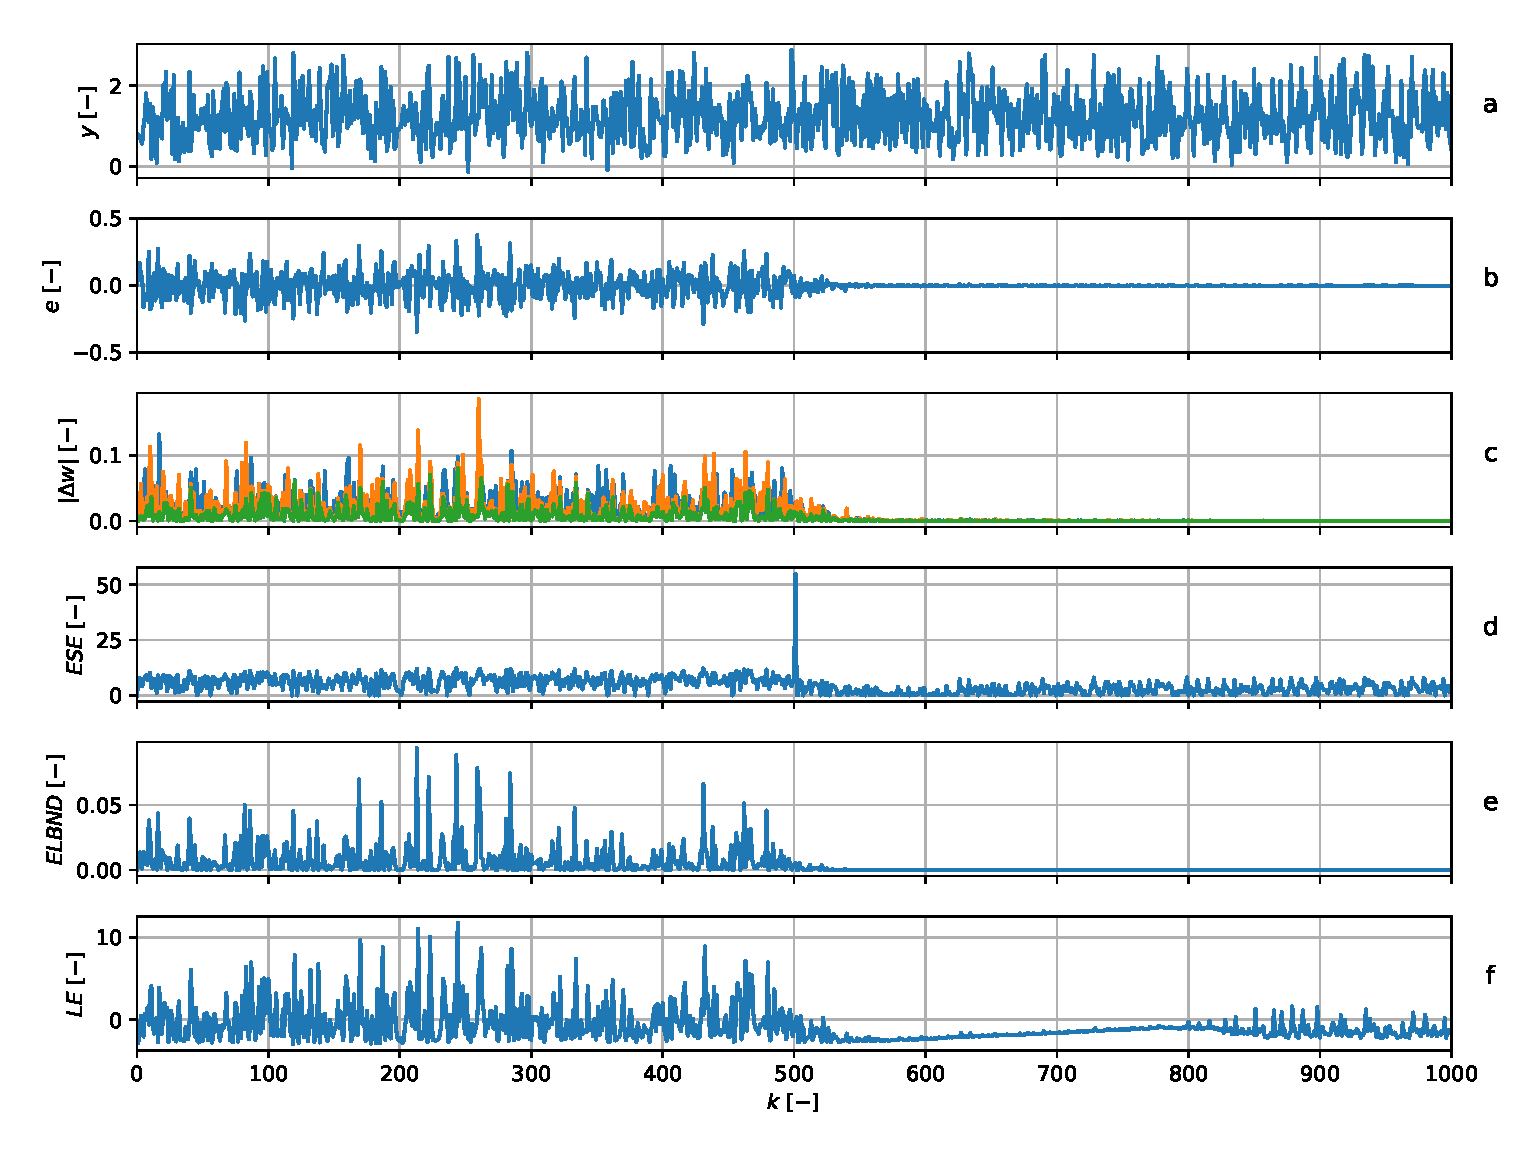
\includegraphics[scale=0.6]{IMG/mdpi/noise_ext.eps} 
    \caption{Detekce vymizení šumu ze signálu. Na grafu (a) je zobrazena původní časová řada (modrá). Graf (b) zobrazuje chybu filtru $e$. Na grafu (c) jsou zobrazeny velikosti přírůstků adaptivních vah filtru. Na grafu (d) jsou pak výsledky modifikovaného algoritmu ESE, přičemž k odstranění šumu ze signálu došlo v diskrétní časový okamžik $k=500$. Je tedy vidět globální maximum v ESE odpovídající úspěšné detekci vymizení šumu ze signálu. Na grafech (e) a (f) jsou pak výsledky získané pomocí metod ELBND a LE.}
    \label{fig:noise_ext}
\end{figure}

\section{Detekce změny trendu}\label{chap:mdpi_trendchange}
Cílem této kapitoly je demonstrovat použití algoritmu ESE při detekci změny trendu, což je úloha, která se často vyskytuje v oblasti detekce poruch a diagnostice \cite{diagnosis}. Uvažujme opět dva vstupy $x_1(k) \sim U(0,1)$ a $x_2(k)\sim U(0,1)$ a výstup generátoru dat $y(k)$ takový, že
\begin{equation}
    y(k)=x_1(k)+x_2(k)+0.01\cdot k + v(k)
\end{equation}
kde člen $v(k)$ reprezentuje aditivní gaussovský šum s nulovou střední hodnotou a směrodatnou odchylkou $\sigma_n=0.1$. V diskrétním časovém okamžiku $k=500$ nastane změna trendu. Výstup generátoru signálu se změní, tak, že
\begin{equation}
     y(k)=x_1(k)+x_2(k)+0.0105 \cdot k + v(k),
\end{equation}
pro $k\geq 500$. 
\par
Pro zpravování signálu byl použit filtr typu LNU s třemi vstupy, takže výstup uvedeného filtru je ve tvaru
\begin{equation}
    \hat{y}(k)=w_1\cdot x_1(k)+w_2\cdot x_2(k)+w_3
\end{equation}
takže odpovídající vektor vstupů je
\begin{equation}
    \textbf{x}(k)=[x_1(k),x_2(k),1].
\end{equation}
Struktura LNU byla vybrána tak, aby co nejlépe odpovídala struktuře generátoru signálu. Parametry adaptivního filtru byly v tomto experimentu adaptovány algoritmem GNGD. Rychlost učení byla nastavena na $\mu=1$, délka okna byla $n_s=500$ a POT metoda byla zvolena podle \ref{eq:l1}. Na obrázku \ref{fig:trend_change} jsou zobrazeny výsledky experimentu. Globální maximum ESE odpovídá okamžiku změny trendu. Algoritmy LE a ELBND úspěšně změnu trendu také detekovali. Pro výpočet LE byl použit vztah \ref{eq:le_direct_padasip} a délka okna byla nastavena na $M=300$. Výpočet ELBND byl proveden podle rovnice \ref{eq:elbnd2}.

\begin{figure}[ht!]

    \centering
    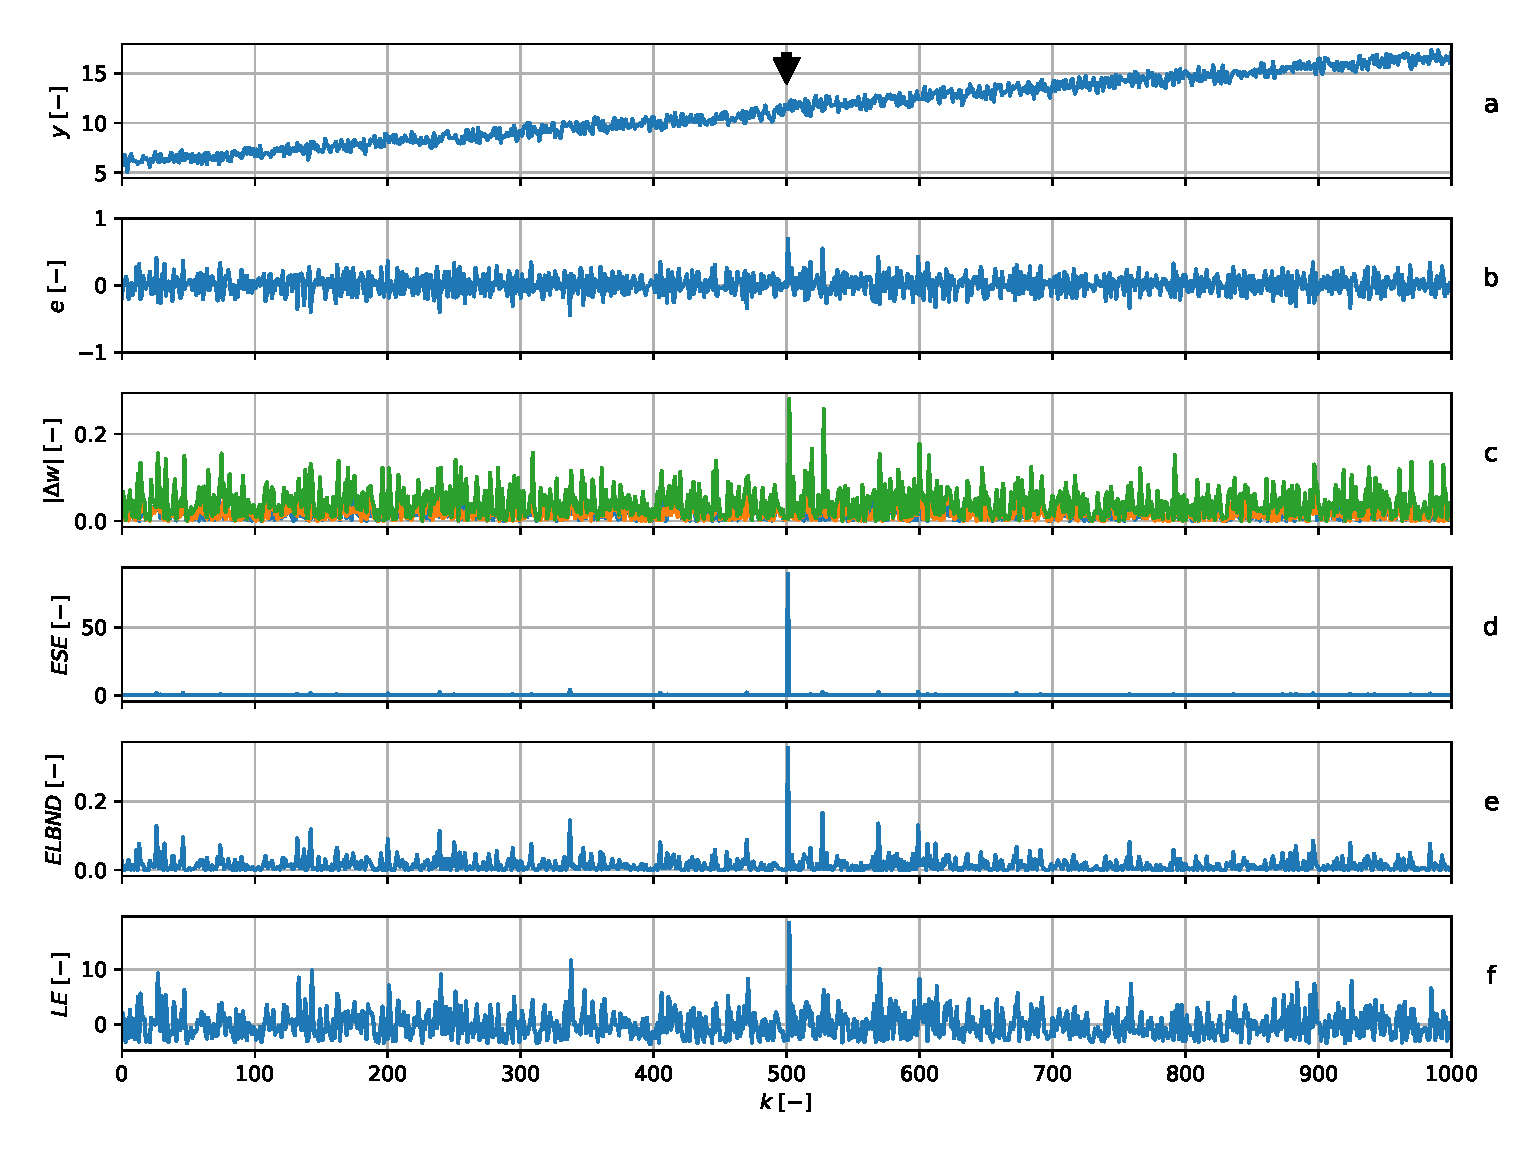
\includegraphics[scale=0.60]{IMG/mdpi/trendchange.eps}
    \caption{Detekce změny trendu při použití algoritmu GNGD. Na grafu (a) jsou zobrazena data z generátoru signálu (modré). Černá šipka znázorňuje okamžik ve kterém došlo ke změně trendu. Na grafu (b) je zobrazena chyba adaptivního filtru $e$. Na grafu (c) jsou znázorněny velikosti přírůstků adaptivních vah filtru. Grafy (d), (e) a (f) znázorňují výsledky detekce novosti pomocí algoritmů ESE, ELBND a LE. Všechny tři algoritmy vykazují úspěšnou detekci změny trendu, která koresponduje s jejich maximální hodnoty během experimentu.}
\label{fig:trend_change}
\end{figure}
\par
Vzhledem k tomu, že pro algoritmus ESE není důležité, jaký konkrétní adaptivní algoritmus je použit, jsou na následujících obrázcích ještě zobrazeny výsledky detekce změny trendu s použitím algoritmů RLS (viz obrázek \ref{fig:trend_change_rls}) a LMS (viz obrázek \ref{fig:trend_change_lms}). Pro algoritmus RLS bylo prvotní nastavení parametru $\delta=10$, pro algoritmus LMS byla nastavena rychlost učení $\mu=0.1$. Výsledky těchto dvou algoritmů publikovány nebyly.

\begin{figure}[ht!]
\centering
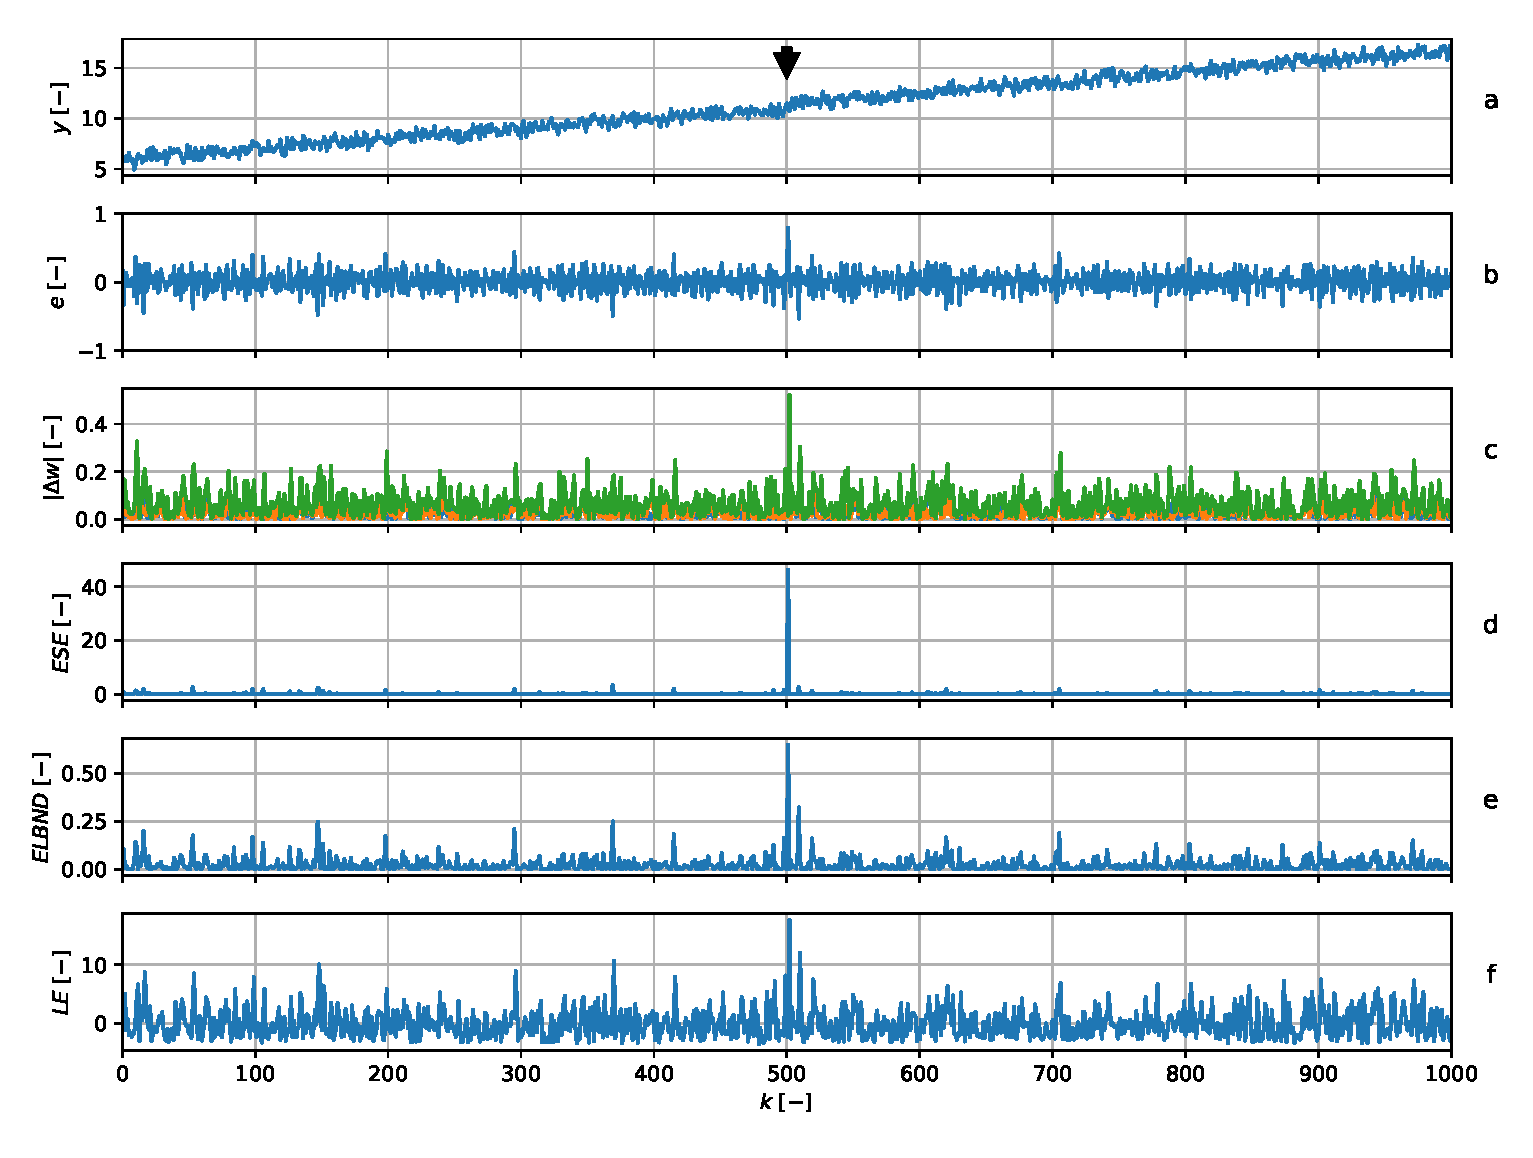
\includegraphics[scale=0.60]{IMG/mdpi/trendchange_rls.eps}
\caption{Detekce změny trendu při použití algoritmu RLS. Na grafu (a) jsou zobrazena data z generátoru signálu (modré). Černá šipka znázorňuje okamžik ve kterém došlo ke změně trendu. Na grafu (b) je zobrazena chyba adaptivního filtru $e$. Na grafu (c) jsou znázorněny velikosti přírůstků adaptivních vah filtru. Grafy (d), (e) a (f) znázorňují výsledky detekce novosti pomocí algoritmů ESE, ELBND a LE. Všechny tři algoritmy vykazují úspěšnou detekci změny trendu, která koresponduje s jejich maximální hodnoty během experimentu.}
\label{fig:trend_change_rls}
\end{figure}

\begin{figure}[ht!]
    \centering
    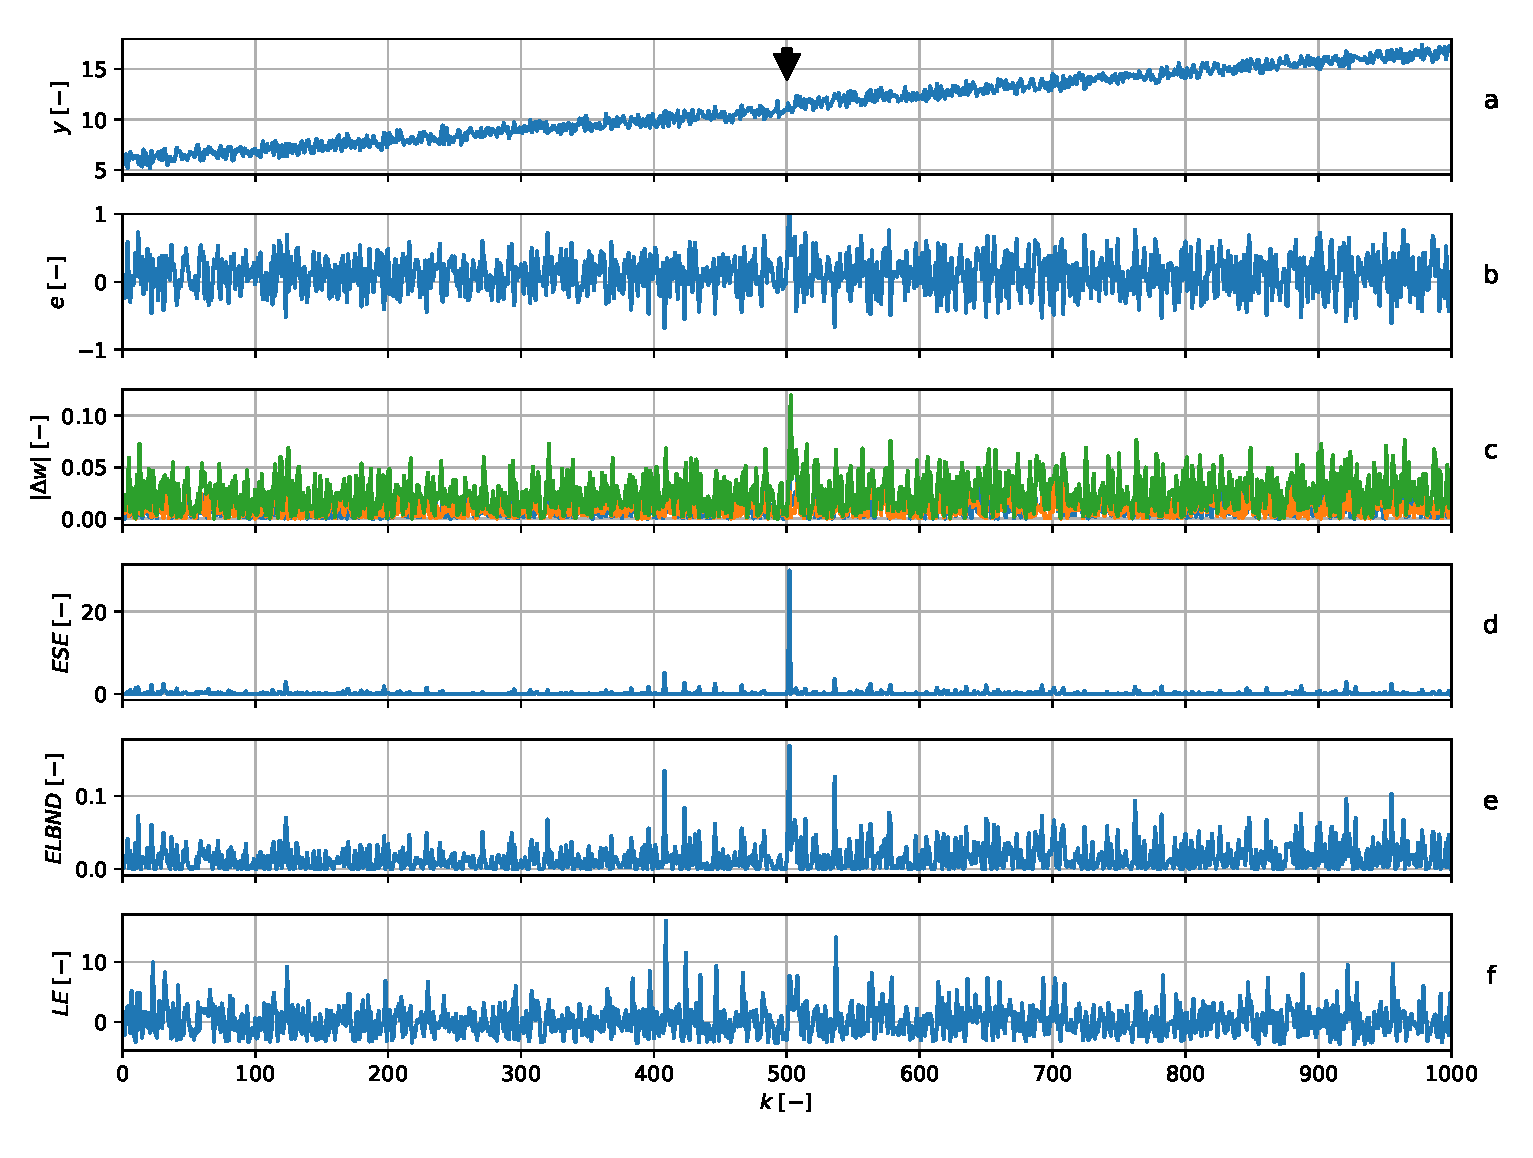
\includegraphics[scale=0.60]{IMG/mdpi/trendchange_lms.eps}
    \caption{Detekce změny trendu při použití algoritmu LMS. Na grafu (a) jsou zobrazena data z generátoru signálu (modré). Černá šipka znázorňuje okamžik ve kterém došlo ke změně trendu. Na grafu (b) je zobrazena chyba adaptivního filtru $e$. Na grafu (c) jsou znázorněny velikosti přírůstků adaptivních vah filtru. Grafy (d), (e) a (f) znázorňují výsledky detekce novosti pomocí algoritmů ESE, ELBND a LE. Všechny tři algoritmy vykazují úspěšnou detekci změny trendu, která koresponduje s jejich maximální hodnoty během experimentu.}
\label{fig:trend_change_lms}
\end{figure}
\section{Detekce epilepsie v záznamu myšího EEG}\label{chap:mdpi_eeg}
Poslední případová studie je věnována detekci epileptického záchvatu v signálu EEG myši pomocí algoritmu EEG. Standartizovaná data ze tří vybraných kanálů EEG, ve kterých byl expertem stanoven začátek epileptického záchvatu přibližně v čase $k \approx 1700$, jsou zobrazeny na obrázku \ref{fig:eeg_seizure}. Standartizace byla provedena podle předpisu
\begin{equation}
y=\frac{x-\mu_{x}}{\sigma_{x}}
\end{equation}
kde $y$ je výsledná standartizovaná hodnota, $x$ je původní hodnota, $mu_x$ je průměrná hodnota původních dat daného kanálu a $\sigma_x$ je jejich původní směrodatná odchylka.
\par
Jako adaptivní filtr byl, na základě experimentů, zvolen FIR filtr délky 10. Vstupem je vektor dat
\begin{equation}
\textbf{x}=[x(k-1_,x(k-2),\dots,x(k-10)]
\end{equation}
takže filtr má 10 adaptivních parametrů. Filtr byl adaptován algoritmem NLMS. Rychost učení byla během experimentu nastavena na $\mu=1$. Metoda POT byla zvolena podle vztahu \ref{eq:l3} a délka okna $n_s=1000$. Výsledky detekce algoritmem ESE jsou zobrazeny na obrázku \ref{fig:mouse_novelty}. Pozice globálního maxima ESE v kanálu C3 (obzvláště signifikantní) je v diskrétním časovém okamžiku $k=1735$, v kanálu Pz je to  $k=1698$ a v kanálu Fp1 je to v $k=1727$. 

\begin{figure}[ht!]
    \centering
    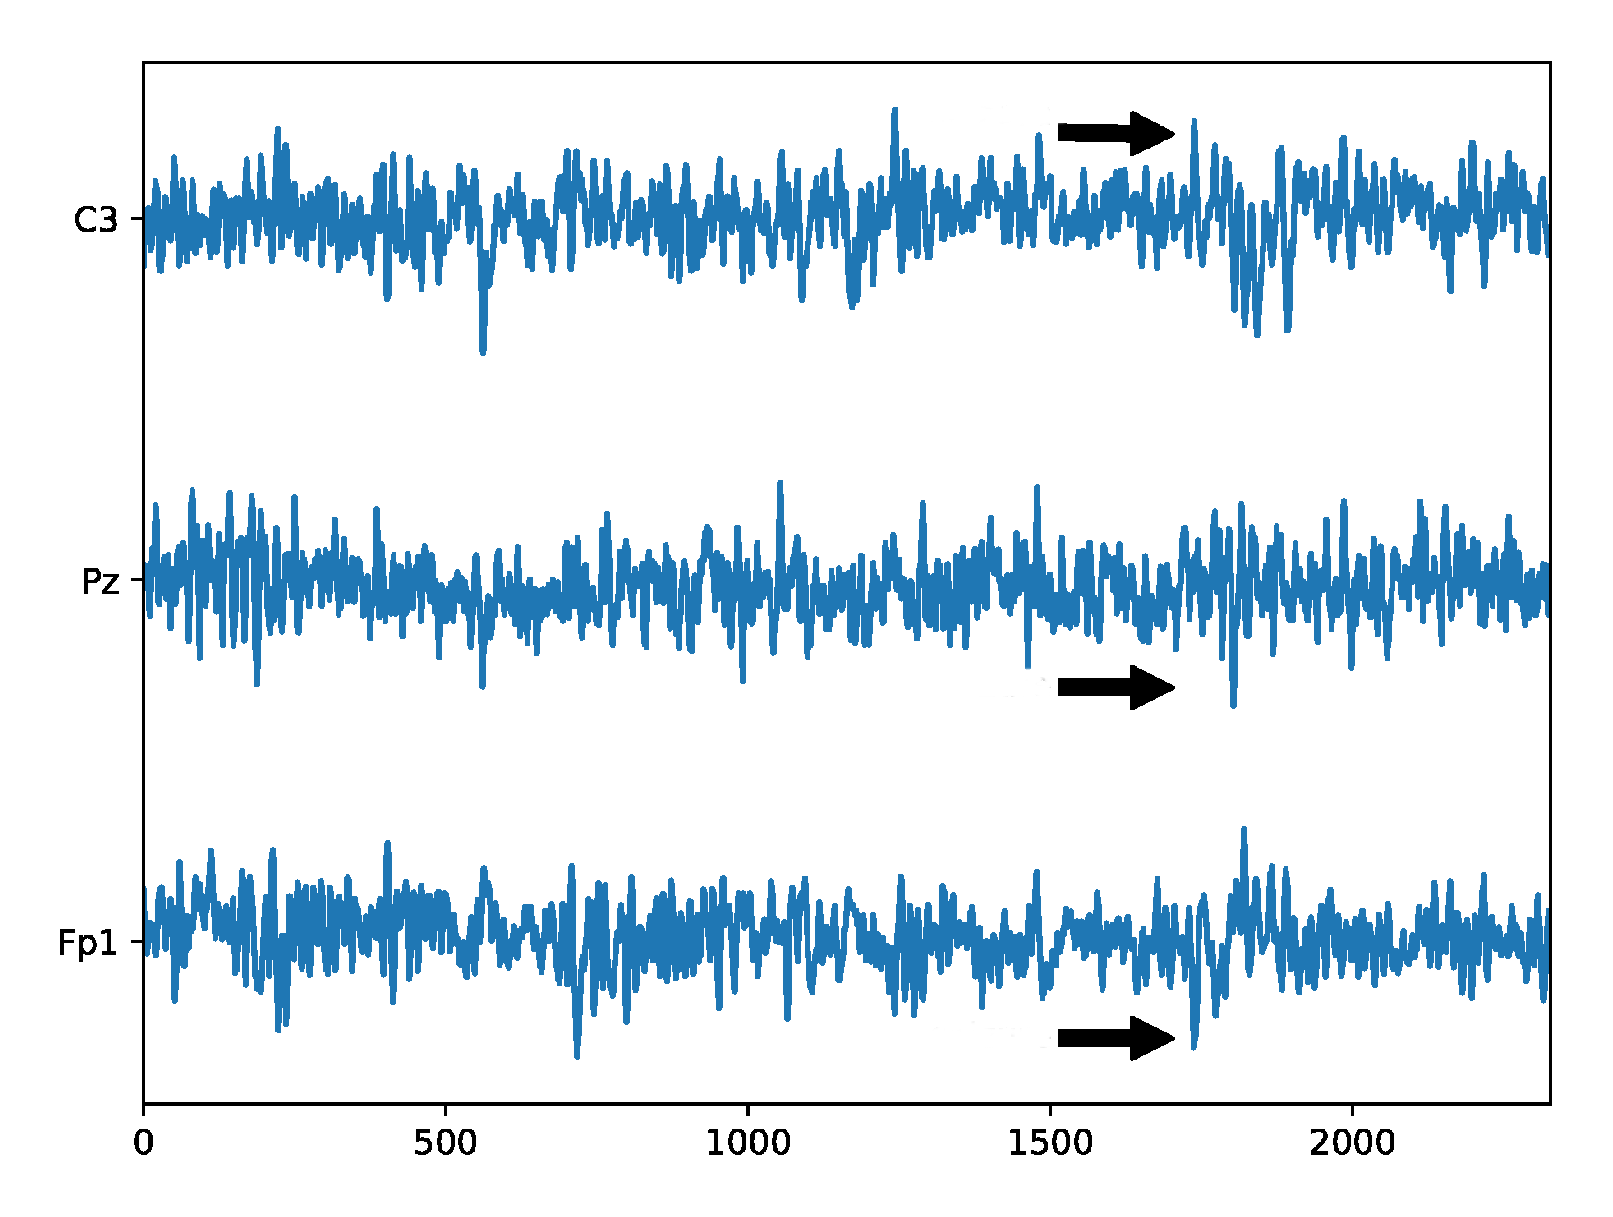
\includegraphics[scale=0.88]{IMG/mdpi/mouse_eeg.eps}
    \caption{Vybrané kanály myšího EEG na kterých je patrný epileptický záchvat. Data byly standartizovány. Začátek záchvatu je přibližně v $k\approx 1700$, což znázorňuje černá šipka.}
    \label{fig:eeg_seizure}
\end{figure}
\begin{figure}[ht!]
    \centering
    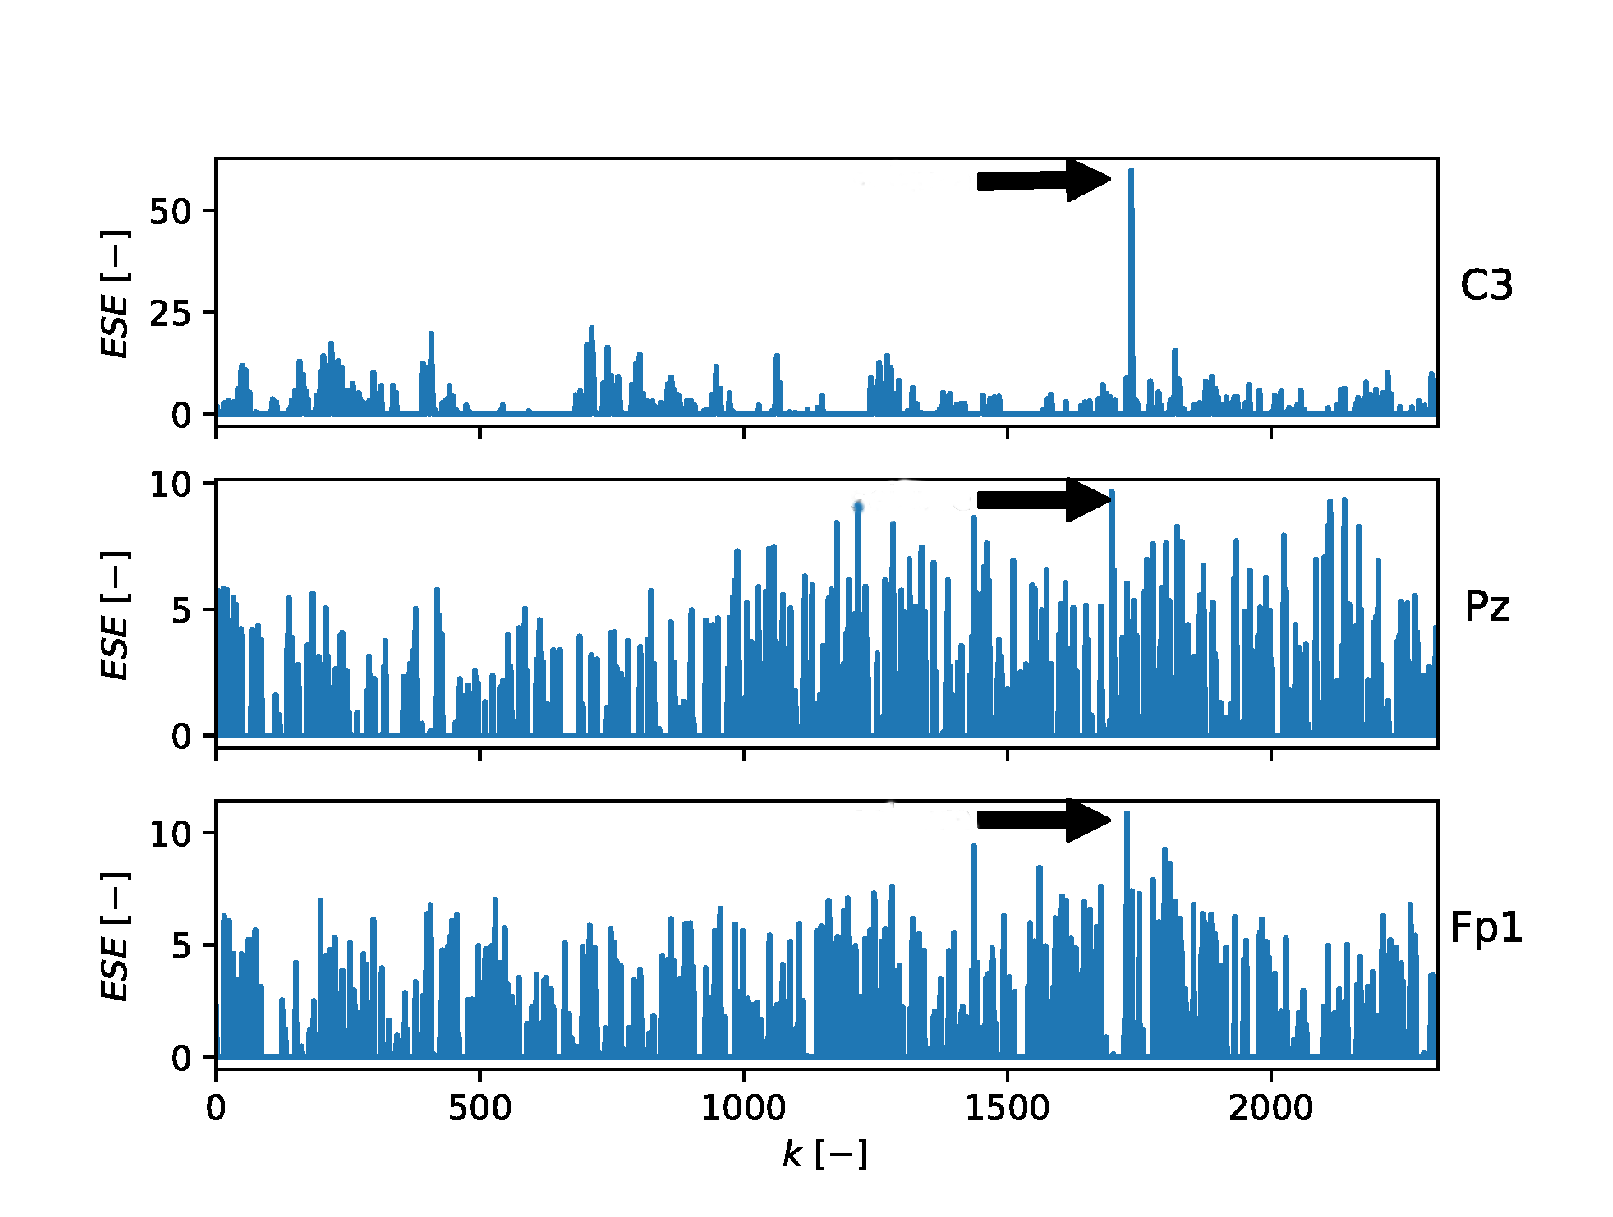
\includegraphics[scale=0.58]{IMG/mdpi/mouse_novelty.eps}
    \caption{Hodnota ESE pro vybrané kanály se záznamem myšího EEG ve kterých je patrný epileptický záchvat. V kanále C3 je v ESE výrazný nárůst po začátku záchvatu (přibližně v $k \approx 1700$), v porovnání s ostatními kanály. Černá šipka znázorňuje přibližný začátek epileptického záchvatu.}
    \label{fig:mouse_novelty}
\end{figure}


\section{Vyhodnocení úspěšnosti detekce skokové změny parametrů generátoru signálu}\label{chap:mdpi_step_stats}
Pro vyhodnocení úspěšnosti skokové změny parametrů generátoru signálu uvažujme generátor signálu s dvěma vstupy $x_1(k)$ a $x_2(k)$ a výstupem $y(k)$ ve tvaru
\begin{equation}
y(k)=a_1\cdot x_1(k)+a_2\cdot x_2(k)+a_3\cdot x_1(k) \cdot x_2(k)+v(k)
\end{equation}
kde člen $v(k)$ reprezentuje gaussovský aditivní šum s nulovou střední hodnotou a směrodatnou odchylkou $\sigma$. Počáteční hodnoty parametrů $a_1$, $a_2$ a $a_3$ jsou vygenerovány z rovnoměrného rozdělení $U(-1,1)$. V diskrétním časovém okamžiku $k=200$, dojde ke skokové změně těchto parametrů a jejich nová hodnota je opět náhodně vygenerována z rovnoměrného rozdělení $U(-1,1)$. Celkový počet vzorků experimentu je 400.
Použitý adaptivní filtr je stejný jako v předchozí případové studii detekce skokové změny parametrů generátoru signálu, viz kapitola \ref{chap:mdpi_stepchange}. Parametry tohoto adaptivního filtru byly adaptovány algoritmem GNGD. Metoda POT byla zvolena podle rovnice \ref{eq:l1} a délka okna byla zvolena $n_s=1200$. Apriorní informace o parametrech GPD byla pro každý experiment získána pomoci 1200 vzorků, s počátečními hodnotami parametrů $a_1$, $a_2$ a $a_3$. Pro každý experiment byla vyhodnocena hodnota SNR jako
\begin{equation}\label{eq:snr}
SNR=10\log_{10}\frac{\sigma_s^2}{\sigma^2}
\end{equation}
kde $\sigma_s$  je hodnota směrodatné odchylky výstupu generátoru signálu během experimentu a $\sigma$ je směrodatná odchylka aditivního gaussovského šumu. Vyhodnocení přesnosti detekce bylo provedeno následujícím způsobem:
\begin{enumerate}
\item nastavení hodnoty směrodatné odchylky šumu $\sigma$
\item pro zvolenou hodnotu směrodatné odchylky $\sigma$ se provede 1000 experimentů, přičemž pro každý experiment jsou nově vygenerovány počáteční hodnoty parametrů generátoru signálu $a_1$, $a_2$ a $a_3$.
\item pro každý experiment je vyhodnocena úspěšnost detekce. Za úspěšnou detekci je považováno, pokud globální maximum ESE, ELBND, EL respektive chyby filtru je v mezích $k\geq 200$ a $k\leq 210$. 
\item vypočte se celková úspěšnost detekce pro danou hodnotu směrodatné odchylky (poměr počtu úspěšných detekcí k celkovému počtu experimentů)
\item pro každý experiment se vyhodnotí SNR podle \ref{eq:snr} a pak se pro zvolenou hodnotu $\sigma$ vypočítá průměrná hodnota $SNR$ pro všechny experimenty
\end{enumerate}
Vyhodnocení úspěšnosti detekce bylo vyhodnoceno pro dva případy. V prvním případě, byly hodnoty vstupů $x_1(k)$ a $x_2(k)$ generovány z rovnoměrného rozdělení $U(-1,1)$. Výsledky úspěšnosti detekce pro různé hodnoty směrodatných odchylek šumu $\sigma$ jsou zobrazeny na obrázku \ref{fig:step_uni_stats}. Výsledky jsou také shrnuty v tabulce \ref{tab:uniform} (viz příloha \ref{priloha:tab}). Pro porovnání jsou zvoleny metody ELBND (výpočet podle rovnice \ref{eq:elbnd2}), LE s oknem $n_s=1200$ (výpočet podle rovnice \ref{eq:le_direct_padasip}) a velikost chyby adaptivního filtru $e$ (v grafu označeno jako ERR).

\begin{figure}[!ht]
    \centering
    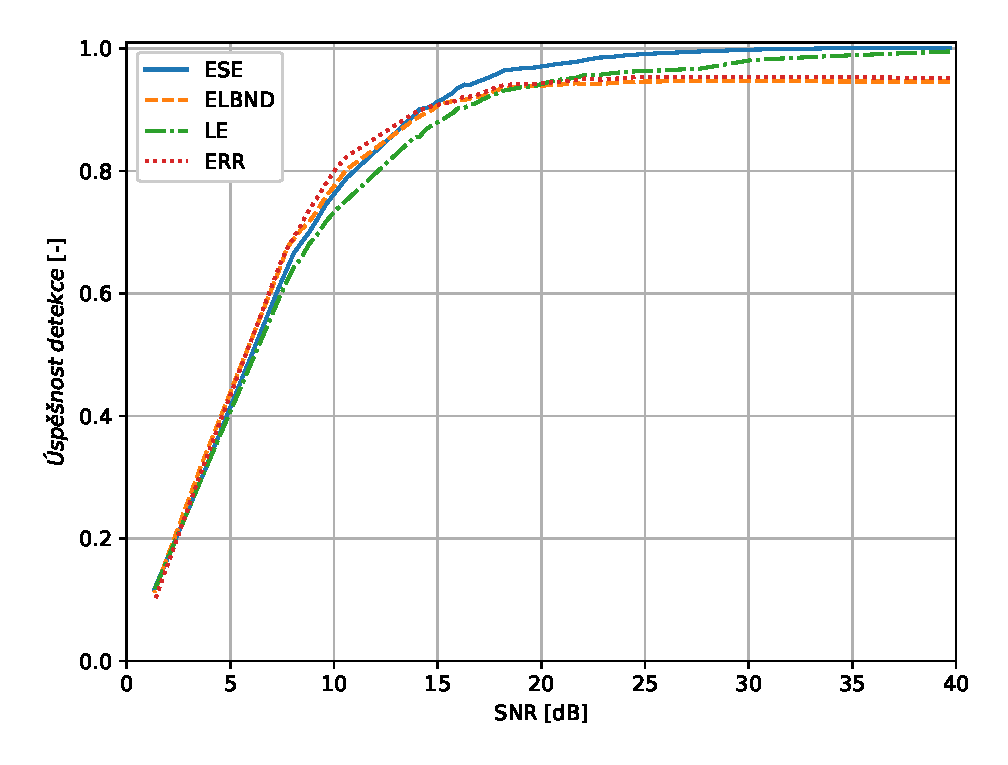
\includegraphics[scale=0.66]{IMG/mdpi/stepuni_stats.eps}
    \caption{Úspěšnost detekce skokové změny parametrů generátoru signálu. Hodnoty vstupů generátoru signálu jsou generovány z rovnoměrného rozdělení $U(-1,1)$. 
Pro hodnoty $SNR > 15$ $dB$ dosáhl algoritmus ESE vyšší úspěšnost než algoritmy  LE, ELBND a vyhodnocení pomocí chyby filtru (ERR). Pro $SNR > 33$ $dB$ dosáhl algoritmus ESE 100\% úspěšnost detekce.}
    \label{fig:step_uni_stats}
\end{figure}
Ve druhém případě byly hodnoty vstupů $x_1(k)$ a $x_2(k)$ generovány z normálního rozdělení. Vyhodnocení úspěšnosti detekce bylo provedeno stejně jako v případě popsaném výše. Výsledky ůspěšnosti detekce pro různé hodnoty směrodatných odchylek šumu $\sigma$ jsou zobrazeny na obrázku \ref{fig:step_norm_stats}. Uvedené výsledky v číselné podobě jsou uvedeny v tabulce \ref{tab:normal} (viz příloha \ref{priloha:tab}). Výpočet hodnot ELBND, LE a ERR bylo provedeno stejně jako ve výše uvedeném případě.

\begin{figure}[!h]
    \centering
    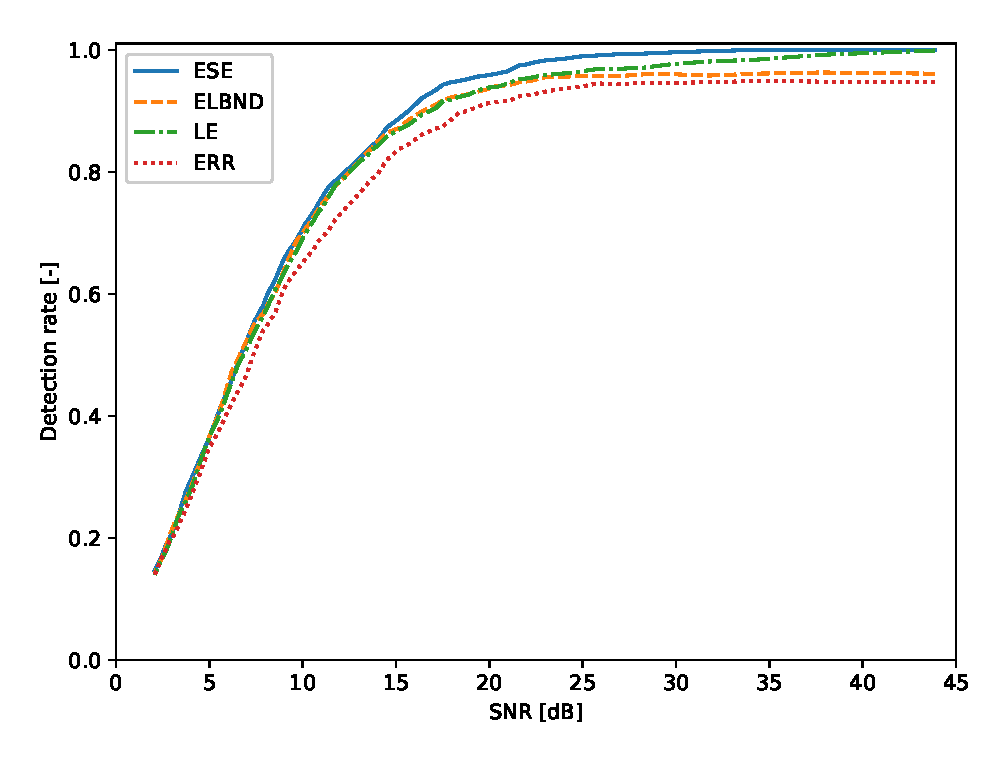
\includegraphics[scale=0.66]{IMG/mdpi/stepnorm_stats.eps}
    \caption{Úspěšnost detekce skokové změny parametrů signálu. Hodnoty vstupů generátoru signálu jsou generovány z normálního rozdělení $N(0,1)$. Pro hodnoty $SNR > 8$ $dB$ dosáhl algoritmus ESE  lepší úspěšnosti detekce než algoritmy LE, ELBND a vyhodnocení pomocí velikosti chyby predikce (ERR). Pro $SNR > 34$ $dB$ dosáhl algoritmus ESE 100\% úspěšnosti detekce.}
    \label{fig:step_norm_stats}
\end{figure}


\section{Vyhodnocení úspěšnosti detekce skokové změny trendu}\label{chap:mdpi_trendchange_evaluation}
Pro vyhodnocení úspěšnosti změny trendu uvažujme výstup generátoru signálu $y(k)$ se dvěma vstupy $x_1(k)$ a $x_2(k)$ jehož výstup je definován jako
\begin{equation}\label{eq:trnd_stats}
    y(k) = x_1(k) + x_2(k) + 0.01 \cdot k + v(k)
\end{equation}
kde člen $v(k)$ reprezentuje aditivní gaussovký šum s nulovou střední hodnotou a směrodatnou odchylkou $\sigma$. V diskrétním časovém okamžiku $k=200$ se změní výstup generátoru signálu
\begin{equation}
    y(k) = x_1(k) + x_2(k) + (0.01 + a) \cdot k + v(k)
\end{equation}
přičemž parametr $a$ je vygenerován v každém experimentu z rovnoměrného rozdělení $U(-0.02,0.02)$. Počet vzorků experimentu je 400.
\par 
Struktura adaptivního filtru byla zvolena stejně jako v předcházející případové studii detekce změny trendu (viz kapitola \ref{chap:mdpi_stepchange}). Adaptivní parametry filtru byly adaptovány algoritmem GNGD. Metoda POT pro algoritmus ESE byla zvolena jako \ref{eq:l1} a délka okna byla nastaven na $n_s=1200$. Apriorní informace o parametrech GPD byla získána na základě 1200 vzorků, ve kterých nedošlo ke změně trendu. 
\par 
Vyhodnocení přesnosti detekce změny trendu bylo provedeno následujícím způsobem:
\begin{enumerate}
\item nastavení hodnoty směrodatné odchylky šumu $\sigma$
\item pro zvolenou hodnotu směrodatné odchylky $\sigma$ se provede 1000 experimentů. V každém experimentu dojde v diskrétním časovém okamžiku $k=200$ k  novému vygenerování hodnoty parametru $a$ z rovnoměrného rozdělení $U(-0.02,0.02)$.
\item pro každý experiment je vyhodnocena úspěšnost detekce. Za úspěšnou detekci je považováno, pokud globální maximum ESE, ELBND, EL respektive chyby filtru je v mezích $k\geq 200$ a $k\leq 210$. 
\item vypočte se celková úspěšnost detekce pro danou hodnotu směrodatné odchylky (poměr počtu úspěšných detekcí k celkovému počtu experimentů)
\item pro každý experiment se vyhodnotí SNR podle \ref{eq:snr} a pak se pro zvolenou hodnotu $\sigma$ vypočítá průměrná hodnota $SNR$ pro všechny experimenty
\end{enumerate}

Vyhodnocení úspěšnosti detekce změny trendu bylo vyhodnoceno pro hodnoty vstupů $x_1(k)$ a $x_2(k)$ vygenerovány z rovnoměrného rozdělení $U(-1,1)$. Výsledky úspěšnosti detekce pro různé hodnoty směrodatných odchylek šumu $\sigma$ jsou zobrazeny na obrázku \ref{fig:trend_stats}. Výsledky jsou také shrnuty v tabulce \ref{tab:trend} (viz příloha \ref{priloha:tab}). Pro porovnání jsou zvoleny metody ELBND (výpočet podle rovnice \ref{eq:elbnd2}), LE s oknem $n_s=1200$ (výpočet podle rovnice \ref{eq:le_direct_padasip}) a velikost chyby adaptivního filtru $e$ (v grafu označeno jako ERR).

\begin{figure}[!ht]
    \centering
    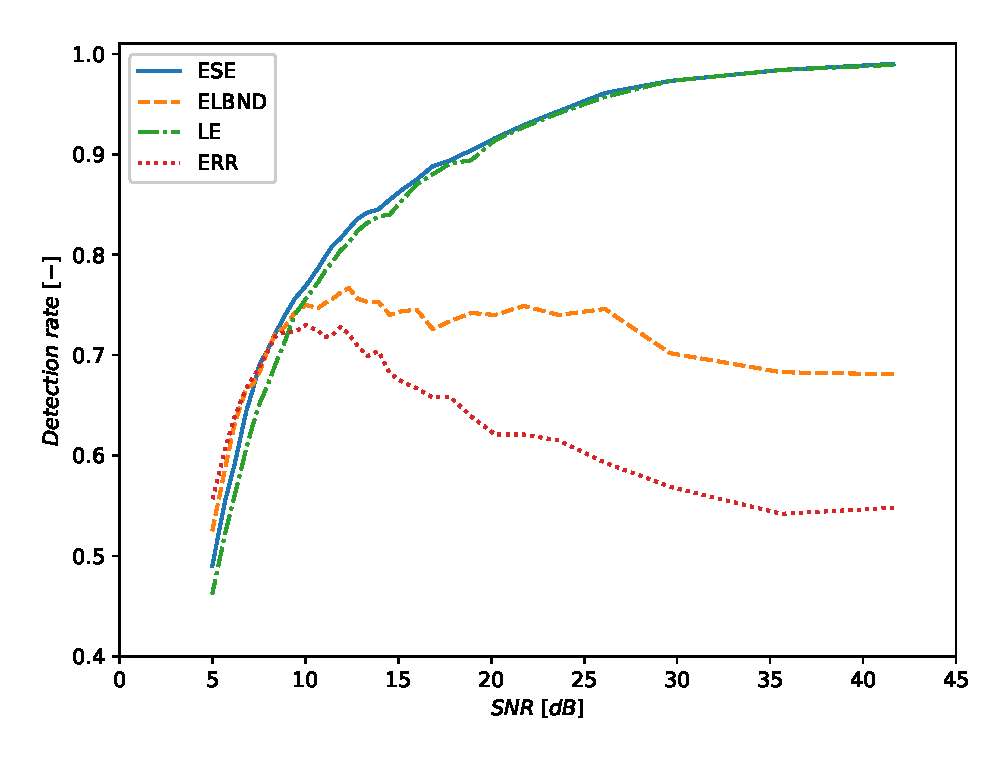
\includegraphics[scale=0.66]{IMG/mdpi/trendchange_stats.eps}
    \caption{Úspěšnost detekce změny trendu. Hodnoty vstupů generátoru signálu byly generovány z rovnoměrného rozdělení $U(-1,1)$. Pro hodnoty $SNR > 8$ $dB$ dosáhl algoritmus ESE větší úspěšnosti detekce než LE, ELBND a vyhodnocení pomocí velikosti chyby filtru.}
    \label{fig:trend_stats}
\end{figure}


\section{Evaluace ROC křivky pro detekci změny trendu}\label{chap:appel_roc}
Protože úspěšná detekce novosti pomocí algoritmu ESE je závislá na volbě hodnoty, od které budeme považovat hodnotu ESE za \textquote{novost}, byl proveden experiment detekce změny trendu a vyhodnocena ROC (Receiver Operating Characteristics) křivka \cite{roc_orig}. ROC křivka poskytuje vhodný způsob jak vizualizovat schopnost binárního klasifikátoru klasifikovat správně data na základě proměnlivé velikosti prahu, který klasifikaci určuje (v případě algoritmu ESE je to hodnota ESE) a zároveň umožňuje objektivně jednotlivé klasifikátory porovnávat \cite{roc_bible} (více viz následující podkapitola \ref{chap:roc_specs}). Pro porovnání algoritmu ESE byly opět zvoleny algoritmy LE, ELBND a klasifikátor, který klasifikuje vzorky náhodně.
\subsection{Popis experimentu}
Stejně jako v případě vyhodnocení přesnosti detekce změny trendu (viz podkapitola \ref{chap:mdpi_trendchange_evaluation}) i v tomto experimentu uvažujeme dva vstupy $x_1(k)$ a $x_2(k)$ výstup generátoru signálu $y(k)$ ve tvaru 
\begin{equation}
    \label{eq:trend}
    d(k)=x_1(k)+x_2(x)+0.01\cdot k + v(k)
\end{equation}
\begin{equation*}
0\leq k < 200
\end{equation*}
kde člen $v(k)$ reprezentuje gaussovský aditivní šum s nulovou střední hodnotou a směrodatnou odchylkou $\sigma_n$. V diskrétním časovém okamžiku $k=200$ přejde výstup generátoru signálu do tvaru
\begin{equation}
y(k)=x_1(k)+x_2(x)+(0.01 + a)\cdot k + v(k)
\end{equation}
\begin{equation*}
200 \leq k \leq 399
\end{equation*}
přičemž hodnota parametru $a$ je vygenerována z rovnoměrného rozdělení $U(-0.02,0.02)$ a pro všechna $200 \leq k \leq 399$ je během daného experimentu konstantní. Hodnoty vstupů $x_1(k)$ a $x_2(k)$ jsou generovány z rovnoměrného rozdělení $U(-1,1)$. 
\par 
Jako adaptivní filtr byl zvolen QNU, jehož struktura odpovídá struktuře generátoru signálu. Výstup adaptivního filtru je ve tvaru
\begin{equation}
\hat{y}(k)=w_1\cdot x_1(k)+w_2\cdot x_2(k) + w_3 \cdot x_1(k) \cdot x_2(k)
\end{equation}
a parametry toho adaptivního filtru byly adaptovány algoritmem GNGD. Rychlost učení během experimentů byla nastavena na $\mu=0.5$.
\par 
Apriorní hodnota parametrů GPD pro algoritmus ESE je získána pomocí 1200 vzorků, získaných z výstupu generátoru signálu, který je dán rovnicí \ref{eq:trend}. Během experimentů byla délka okna $n_s=1200$. Metoda POT byla zvolena podle \ref{eq:l1}. Pro výpočet ELBND byl použit vztah \ref{eq:elbnd2}. Výsledky algoritmu LE byly získány pro okno délky $M=1200$ pomocí vztahu \ref{eq:le_direct_padasip}. Pro každou hodnotu $\sigma$ bylo provedeno 10000 experimentů na jejichž základě byla zkonstruována ROC křivka. Hodnoty směrodatných odchylek $\sigma$ byly vybrány takto:
\begin{equation}
\sigma=\{0.1,0.2,0.5,1.0,2.0,2.5 \}
\end{equation}
a pro každou hodnotu $sigma$ byla pro všech 10000 experimentů určená průměrná hodnota $SNR$, která byla pro každý experiment vypočtena podle rovnice $\ref{eq:snr}$. 

\subsection{Konstrukce ROC křivky}\label{chap:roc_specs}
Pro konstrukci ROC křivky je důležité, aby množina výsledků byla vyvážená. Tedy aby obsahovala stejný počet pozitivních i negativních vzorků. Pro získání vyvážené množiny výsledků byl nejdřív každý experiment převzorkován podle následujícího předpisu
\begin{equation}
    ND_r(i) = max\{ND(i \cdot 10), ND(i \cdot 10 + 1), ND(i \cdot 10 + 2), \dots, ND(i \cdot 10 + 9)\}
\end{equation}
\begin{equation*}
i = 0,1,\dots,39
\end{equation*}
kde $ND$ reprezentuje hodnotu detektoru novosti (resp. hodnoty algoritmu ESE, ELBND, LE). Z každé převzorkované datové řady jsou vygenerovány dvě množiny. Množina $P$ obsahuje pozitivní vzorek, takový, že $P=\{ND_r(20)\}$ (protože v diskrétním časovém okamžiku $k=200$ došlo ke změně trendu).  Množina $N$ obsahuje obsahuje zbylých 39 negativních vzorků, takže $N=\{ND(0), \dots ND(19), ND(21), \dots ND(39) \}$. Při konstrukci ROC křivky jsou pro každý experiment vybrány dva vzorky. Jeden vzorek z množiny $P$ a jeden náhodně vybraný vzorek z množiny $N$. Pro vyhodnocení ROC je klíčové zjistit, jestli jsou pozitivní vzorky (prvky množiny $P$) pro daný práh správně klasifikovány jako pozitivní (True Positive) a zda-li jsou negativní vzorky klasifikovány jako falešně pozitivní (False Positive). Pro danou velikost prahu se určí úspěšnost detekce skutečně pozitivních (True Positive Rate) jako 
\begin{equation}
TPR=\frac{TP}{P}=\frac{TP}{10000}
\end{equation}
kde $TP$ je počet správně pozitivně klasifikovaných vzorků a $P$ je celkový počet skutečně pozitivních vzorků. Dále je potřeba určit poměr falešně pozitivních (False Positive Rate) vzorků pro daný práh jako
\begin{equation}
FPR=\frac{FP}{N}=\frac{FP}{10000}
\end{equation}
kde $FP$ je počet vzorků klasifikovaných jako falešně pozitivní a $N$ je celkový počet skutečně negativních vzorků. ROC pak zobrazuje závislost úspěšnost detekce skutečně pozitivních vzorků ($TPR$) v závislosti na poměru falešně pozitivních vzorků ($FPR$).
\par 
Hodnota $TPR$ bývá nazývána také jako sensitivita. Komplementární hodnotou k $FPR$ je potom specifita (True Negative Rate $TNR$), která určuje, kolik opravdu negativních vzorku ($TN$) je klasifikováno jako negativní. Komplementární ve smyslu
\begin{equation}
TNR=\frac{TN}{N}=1-FPR.
\end{equation} 
Komplementární k sensitivitě je hodnota míry falešně negativních ($FNR$), která určuje poměr falešně negativních k ($FN$) k celkovému počtu pozitivních, tedy
\begin{equation}
FNR=\frac{FN}{P}=1-TPR.
\end{equation}
\par 
Pro každou ROC křivku je možné určit plochu pod touto křivkou AUROC (Area Under ROC), která vypovídá o schopnosti klasifikátoru rozlišovat mezi jednotlivými třídami. Čím větší plocha pod křivkou, tím víc klasifikátor správně klasifikuje pozitivní případy jako pozitivní a negativní případy jako negativní. Plocha AUROC ideálního klasifikátoru bude 1, zatímco plocha nejhoršího možného klasifikátoru bude rovna 0 (tento klasifikátor, ale bude dokonalým klasifikátorem, pokud zaměníme označení negativní třídy za pozitivní). Plocha AUROC náhodného klasifikátoru bude 0.5, neboť tento klasifikátor nedokáže vůbec rozlišovat mezi pozitivními a negativními případy.
\subsection{Výsledky experimentu}
Výsledné ROC křivky pro různé hodnoty $SNR$ jsou zobrazeny v obrázcích \ref{fig:roc_01}-\ref{fig:roc_25}. Modrá čára zobrazuje výsledky algoritmu ESE, zelená tečkovaná čára zobrazuje výsledky algoritmu LE, červená přerušovaná čára výsledky algoritmu ELBND a černá čerchovaná čára zobrazuje výsledky náhodného klasifikátoru. 
\par 
Pro každou ROC křivku byla vypočtena hodnota plochy pod touto křivkou, AUROC, pomocí lichoběžníkové metody, jako
\begin{equation}
AUROC \approx \sum_{j=1}^{n_t} \frac{TPR(FPR(j))+TPR(FPR(j+1))}{2} \cdot(FPR(j+1)-FPR(j))
\end{equation}
kde $n_t$ reprezentuje počet vyhodnocovaných prahů zmenšený o 1. Výsledné plochy pod křivkami ROC jsou pro jednotlivé metody a směrodatné odchylky šumu uvedené v následující tabulce \ref{tab:auroc}. Tučně je zvýrazněna nejvetší hodnota AUROC. Podle uvedených hodnot při průměrném $SNR=35.8$ nejlépe rozlišuje mezi pozitivními a negativními případy algoritmus LE. Pro nižší hodnoty $SNR$ je nejlépe separujícím algoritmem ESE.
\begin{table}[h!]

\caption{$AUROC$ pro detekci změny trendu}
\centering
\begin{tabular}{|l|c|c|c|c|}
\hline
\multicolumn{2}{|l|}{} & \multicolumn{3}{c|}{\textbf{AUROC}} \\ \hline
$\sigma_n$ & \textit{SNR [dB]} & \textit{ESE} & \textit{LE} & \textit{ELBND} \\ \hline
0.1 & 35.8 & 0.9954 & \textbf{0.9952} & 0.8234\\ \hline
0.2 & 30.0 & \textbf{0.9920} & 0.9912 & 0.8299 \\ \hline
0.5 & 21.7 & \textbf{0.9816} & 0.9777 & 0.8288 \\ \hline
1.0 & 16.2 & \textbf{0.9576} & 0.9496 & 0.8263 \\ \hline
2.0 & 10.8 & \textbf{0.9286} & 0.9214 & 0.8397 \\ \hline
2.5 & 9.2 & \textbf{0.9134} & 0.9056 & 0.8446 \\ \hline
\end{tabular}
\label{tab:auroc}
\end{table}
V další tabulce \ref{tab:dr} je uvedená úspěšnost klasifikace, kde za úspěšnou klasifikaci je považován případ, kdy maximální hodnota ESE, ELBND nebo LE během experimentu je v intervalu $200\leq k\leq210$, tedy do deseti vzorků po změně trendu.
\begin{table}[h!]
\caption{Úspěšnost detekce změny trendu}
\centering
\begin{tabular}{|l|c|c|c|c|}
\hline
\multicolumn{2}{|l|}{} & \multicolumn{3}{c|}{\textbf{Úspěšnost detekce}} \\ \hline
$\sigma_n$ & \textit{SNR [dB]} & \textit{ESE} & \textit{LE} & \textit{ELBND} \\ \hline
0.1 & 35.8 & 98.88 & \textbf{98.92} & 60.00 \\ \hline
0.2 & 30.0 & \textbf{98.14} & 98.03 & 59.61 \\ \hline
0.5 & 21.7 & \textbf{95.18} & 95.08 & 59.65 \\ \hline
1.0 & 16.2 & \textbf{90.42} & 89.96 & 57.67 \\ \hline
2.0 & 10.8 & \textbf{81.27} & 78.51 & 57.69 \\ \hline
2.5 & 9.2 & \textbf{75.86} & 71.56 & 57.16 \\ \hline
\end{tabular}
\label{tab:dr}
\end{table}
Tučně jsou zvýrazněny hodnoty nejvyšší úspěšnosti detekce. Z výsledků je patrné, že pro průměrné $SNR=35.8$ má nejvyšší úspěšnost algoritmus LE. Pro nižší hodnoty $SNR$ je algoritmem s nejvyšší úspěšností detekce algoritmus ESE.
\begin{figure}[ht!]
    \centering
    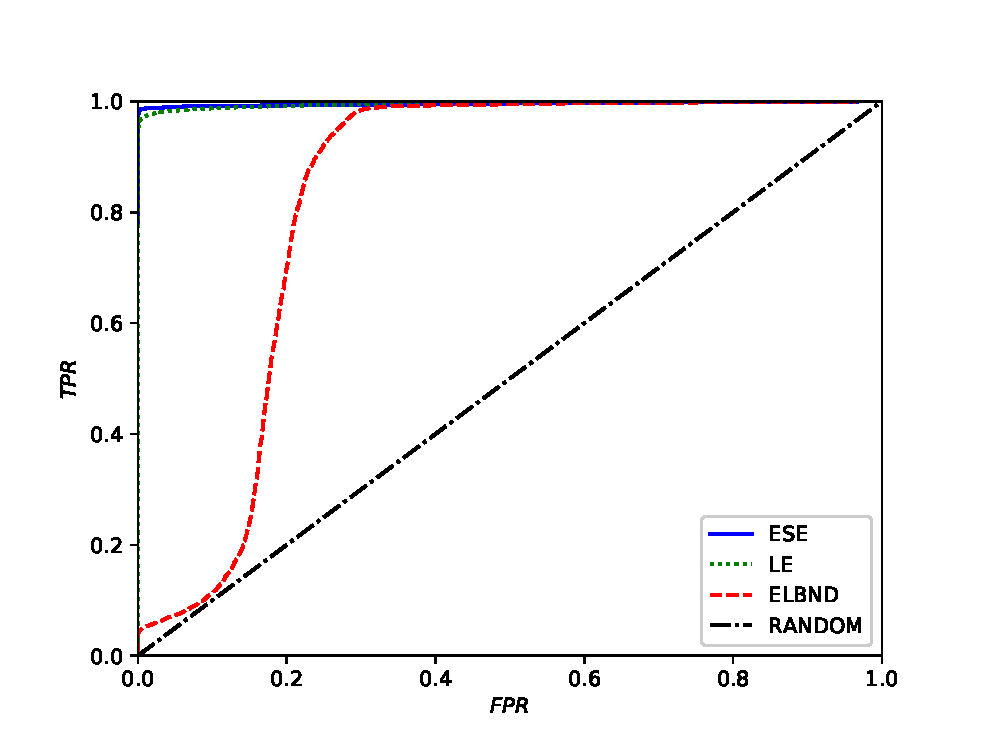
\includegraphics[scale=0.7]{IMG/appel_roc/roc_01.eps}
    \caption{ROC křivky v případě detekce změny trendu signálu obsahujícího aditivní gaussovský šum se směrodatnou odchylkou $\sigma=0.1$. Průměrná hodnota $SNR$ experimentů byla $SNR=35.80$ $dB$. Černá čerchovaná čára (RANDOM) reprezentuje náhodný klasifikátor.}
    \label{fig:roc_01}
\end{figure}
\begin{figure}[ht!]
    \centering
    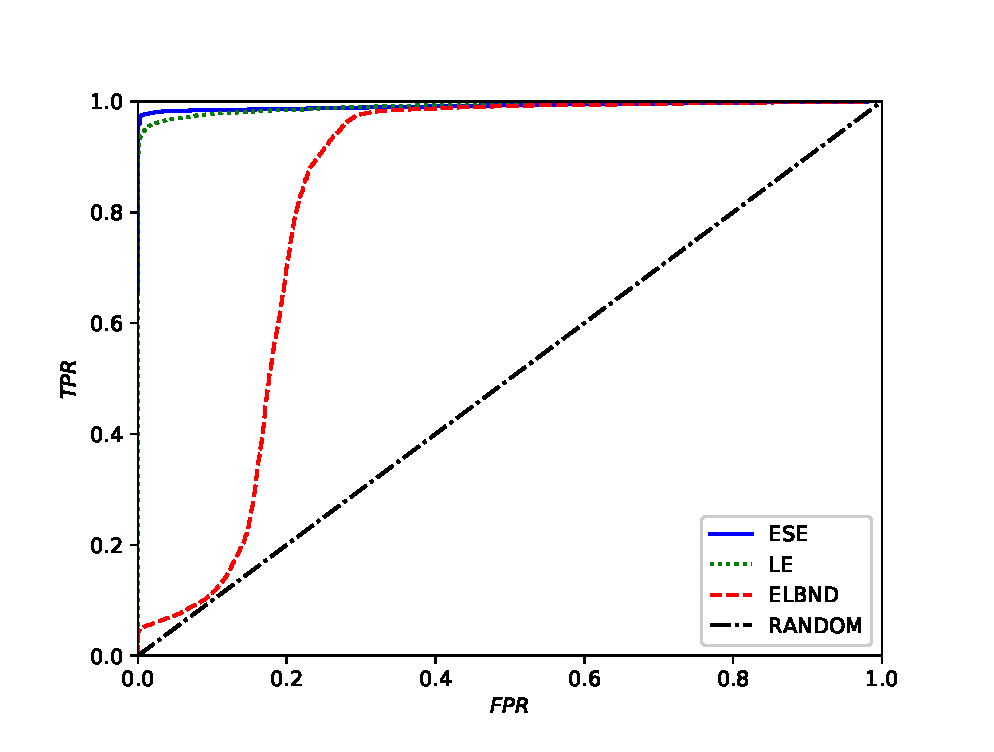
\includegraphics[scale=0.7]{IMG/appel_roc/roc_02.eps}
    \caption{ROC křivky v případě detekce změny trendu signálu obsahujícího aditivní gaussovský šum se směrodatnou odchylkou $\sigma=.2$. Průměrná hodnota $SNR$ experimentů byla $SNR=30.00$ $dB$. Černá čerchovaná čára (RANDOM) reprezentuje náhodný klasifikátor.}
    \label{fig:roc_02}
\end{figure}
\begin{figure}[ht!]
    \centering
    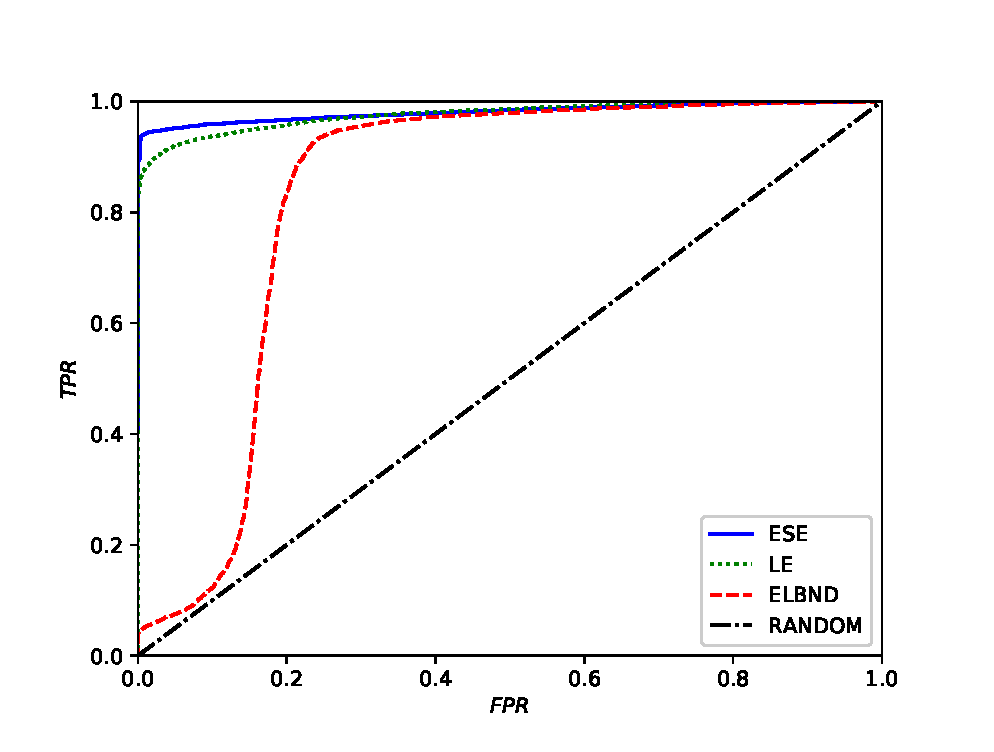
\includegraphics[scale=0.73]{IMG/appel_roc/roc_05.eps}
    \caption{ROC křivky v případě detekce změny trendu signálu obsahujícího aditivní gaussovský šum se směrodatnou odchylkou $\sigma=0.5$. Průměrná hodnota $SNR$ experimentů byla $SNR=21.70$ $dB$. Černá čerchovaná čára (RANDOM) reprezentuje náhodný klasifikátor.}
    \label{fig:roc_05}
\end{figure}
\begin{figure}[ht!]
    \centering
    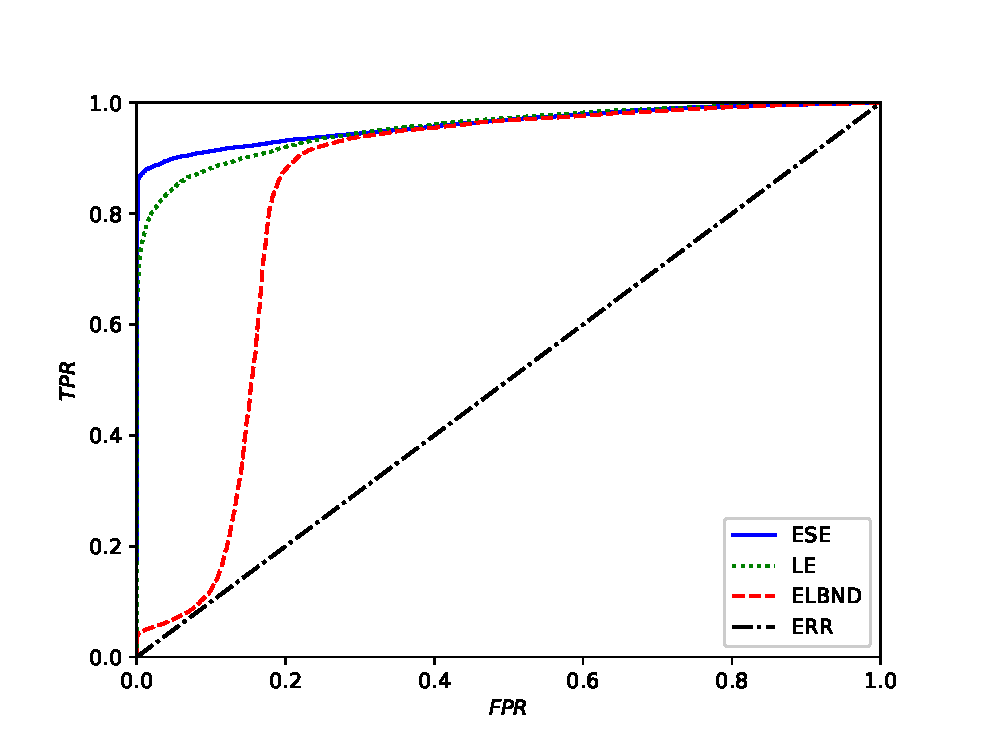
\includegraphics[scale=0.73]{IMG/appel_roc/roc_1.eps}
    \caption{ROC křivky v případě detekce změny trendu signálu obsahujícího aditivní gaussovský šum se směrodatnou odchylkou $\sigma=1.0$. Průměrná hodnota $SNR$ experimentů byla $SNR=16.20$ $dB$. Černá čerchovaná čára (RANDOM) reprezentuje náhodný klasifikátor.}
    \label{fig:roc_1}
\end{figure}
\begin{figure}[ht!]
    \centering
    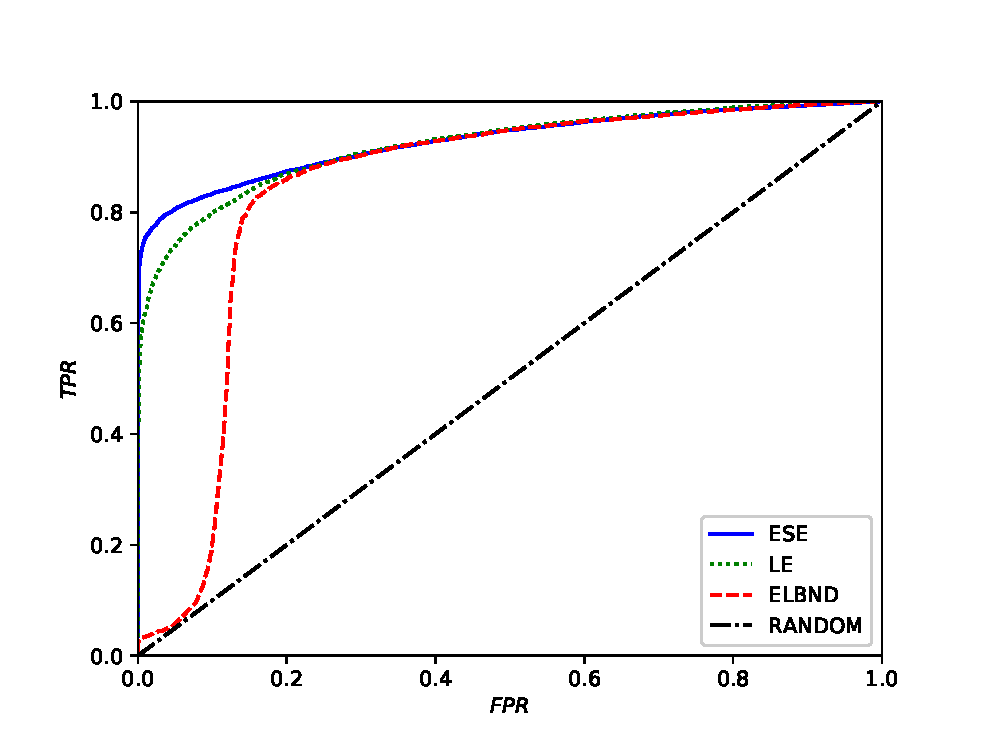
\includegraphics[scale=0.73]{IMG/appel_roc/roc_2.eps}
    \caption{ROC křivky v případě detekce změny trendu signálu obsahujícího aditivní gaussovský šum se směrodatnou odchylkou $\sigma=2.0$. Průměrná hodnota $SNR$ experimentů byla $SNR=10.88$ $dB$. Černá čerchovaná čára (RANDOM) reprezentuje náhodný klasifikátor.}
    \label{fig:roc_2}
\end{figure}
\begin{figure}[ht!]
    \centering
    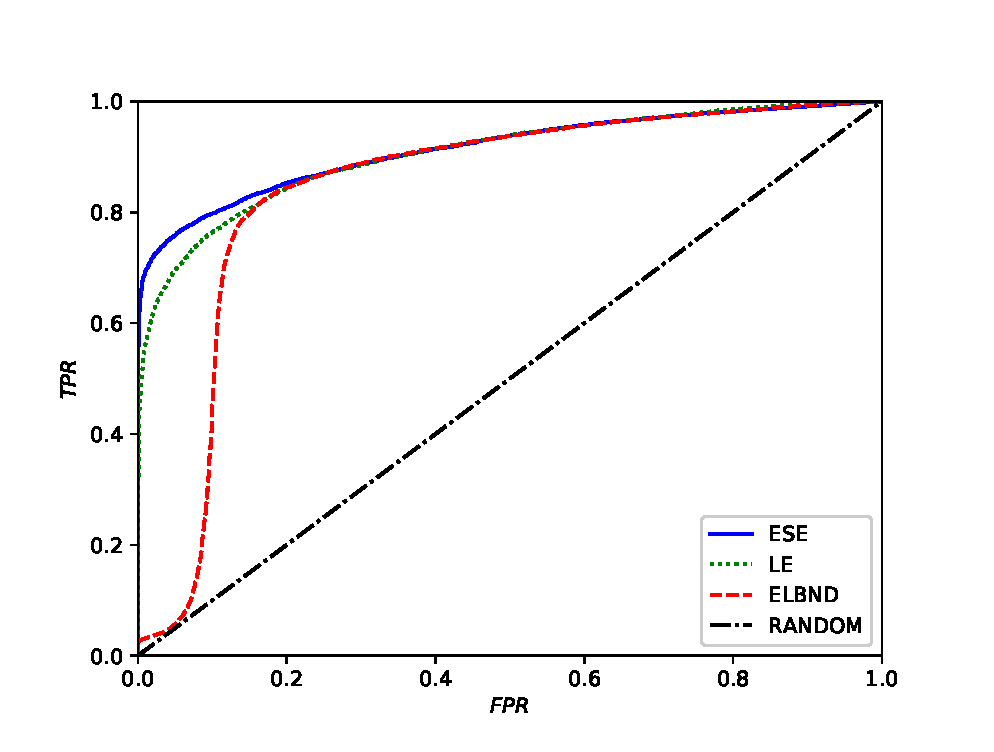
\includegraphics[scale=0.73]{IMG/appel_roc/roc_25.eps}
    \caption{ROC křivky v případě detekce změny trendu signálu obsahujícího aditivní gaussovský šum se směrodatnou odchylkou $\sigma=2.5$. Průměrná hodnota $SNR$ experimentů byla $SNR=9.20$ $dB$. Černá čerchovaná čára (RANDOM) reprezentuje náhodný klasifikátor.}
    \label{fig:roc_25}
\end{figure}

\section{Vyhodnocení výpočetní náročnosti metod odhadu parametrů zobecněného Paretova rozdělení}\label{chap:appel_gpd}
Výsledky v této podkapitole byli publikovány v (můj shit). Cílem bylo určit výpočetní čas výpočtu parametrů GPD v typické aplikaci pro použití algoritmu ESE, který byl, v tomto případě, testován ne experimentu detekce skokové změny parametrů generátoru signálu.
\subsection{Motivace}
Detekce novosti v reálném čase je úloha, která nalézá své uplatnění nejen v oblasti detekci a diagnostiky v průmyslových aplikacích \cite{fault}, ale také např. v detekci narušení počítačových sítí \cite{data_streams} nebo v zabezpečovacích systémech \cite{surveilance}. Další oblastí uplatnění je např. mobilní robotika, která je specifická tím, že robot má k dispozici pouze limitovaný výpočetní výkon \cite{robotics_marslan,robotics}. Pro metody detekce novosti v reálném čase je tedy důležité, aby vynikali dostatečně nízkou výpočetní náročností. Z tohoto důvodu byli otestovány tři různé metody výpočtu parametrů GPD (viz kapitola \ref{chap:gpd}, protože tento výpočet je z hlediska použití algoritmu ESE potenciálně limitující z hlediska využitelnosti v aplikacích detekce v reálném čase. Jmenovitě byli otestovány tyto metody: metoda maximální věrohodnosti (ML), metoda momentů (MOM) a metoda kvazi-maximální věrohodnosti (QML) (více viz kapitola \ref{chap:gpd}). Výpočetní čas potřebný k určení parametrů GPD pomocí těchto metod byl vyhodnocen při experimentu, ve kterém dojde ke skokové změně parametrů generátoru signálu.
\subsection{Specifikace experimentu}
Vzhledem k povaze experimentu, který slouží k vyhodnocení výpočetní náročnosti různých metod určení parametrů GPD, a nikoliv k detekci novosti v nějakém komplexním procesu, byl zvolen jednoduchý lineární kombinační filtr (LNU), jehož výstup v diskrétním časovém okamžiku $k$ je definován jako
\begin{equation}\label{eq:gene_ese_1}
\hat{y}(k)=w_1\cdot x_1(k)+w_2\cdot x_2(k)+w_3\cdot x_3(k)
\end{equation}
a tento filtr je adaptován algoritmem NLMS (viz kapitola \ref{chap:nlms}), přičemž rychlost učení $\mu$ byla nastavena jako $\mu=0.8$.
\par 
Pro výstup generátoru signálu platí vztah
\begin{equation}
y(k)=x_1(k)+x_2(k)+x_3(k)+v(k)
\end{equation}
pro všechny $1 \leq k \leq 200$. Člen $v(k)$ reprezentuje aditivní gaussovský šum s nulovou střední hodnotou a směrodatnou odchylkou $\sigma_{noise}=0.1$. V diskrétním časovém okamžiku $k=201$ dojde ke změně generátoru signálu a jeho výstup přejde do tvaru
\begin{equation}
y(k)=0.7\cdot x_1(k)+1.2\cdot x_1(k)+1.1 \cdot x_1(k) + v(k)
\end{equation}
pro $201 \leq k \leq 400$. Hodnota všech vstupů generátoru signálu je v každém časovém okamžiku $k$ vybrána ze standartního rozdělení normálního rozdělení, takže $i$-tý vstup $x_i\sim \mathcal{N}(0,1)$. Změna parametrů signálu byla vybrána tak, aby nedošlo ke změně střední hodnoty signálu $y(k)$.
\par
Délka okna pro odhad parametrů GPD byla během experimentu nastavena na $n_s=1200$. Metoda POT byla zvolena podle rovnice \ref{eq:l1}. Před experimentem bylo pořízení 1200 vzorků vygenerovaných generátorem signálu definovaným vztahem \ref{eq:gene_ese_1}, na něž byla použita metoda POT, tak aby při experimentu v diskrétní časový okamžik $k=1$ byla hodnota ESE relevantní.
\par
Průběh výstupní hodnoty filtru je zobrazen na obrázku \ref{fig:par_output}, hodnota ESE potom na obrázku \ref{fig:par_ese}. Hodnoty parametrů $\xi$, $\sigma$, $\mu$ GPD, pro všechny tři adaptivní váhy, během experimentu jsou zobrazeny na obrázcích \ref{fig:par_gamma}, \ref{fig:par_sigma} a \ref{fig:par_mu}.
\par
Experiment byl proveden na PC s procesorem Intel(R) Core(TM) i5-7400 se 4mi jádry s taktovací frekvencí 3001 MHz a operační pamětí o velikosti 32 GB. Operační systém byl Windows 10 Pro, 64-bitová verze 10.0.18362. Kód byl napsán v Python 3.6.1 a byly použity knihovny Numpy 1.17.0 a Scipy 1.4.1.


\begin{figure}[h!]

	\centering
	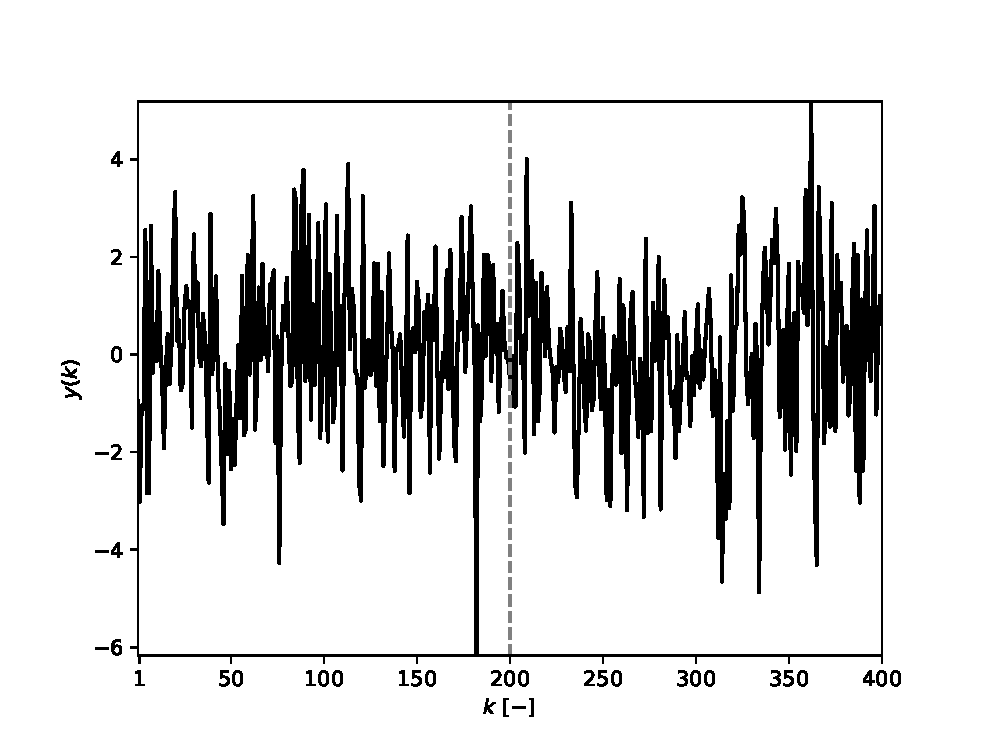
\includegraphics[scale=0.74]{IMG/appel_par/par_output.eps}
	\caption{Výstup adaptivního filtru během experimentu. Skoková změna parametrů generátoru signálu je zvýrazněná svislou vodorovnou čarou v diskrétním časovém okamžiku $k=200$.}
		\label{fig:par_output}
\end{figure}

\subsection{Výsledky a diskuze}


\begin{figure}[h!]

	\centering
	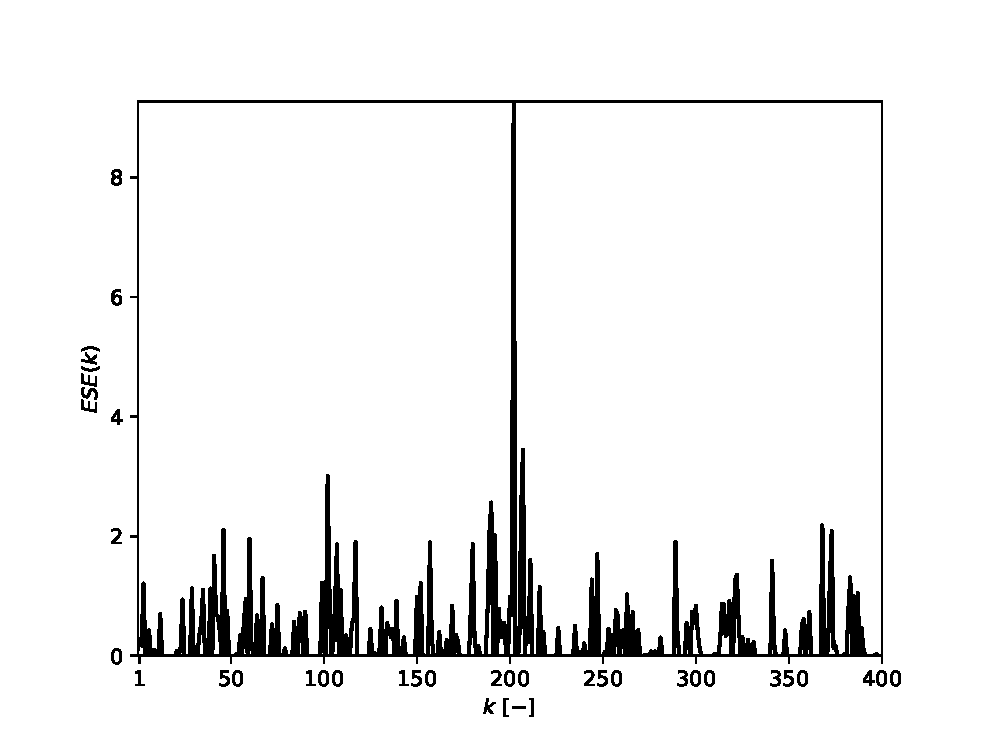
\includegraphics[scale=0.74]{IMG/appel_par/par_ese.eps}
	\caption{Hodnota ESE během experimentu. Globální maximum odpovídá změně parametrů generátoru signálu, resp. úspěšné detekci novosti.}
		\label{fig:par_ese}
\end{figure}

\begin{figure}[h!]

	\centering
	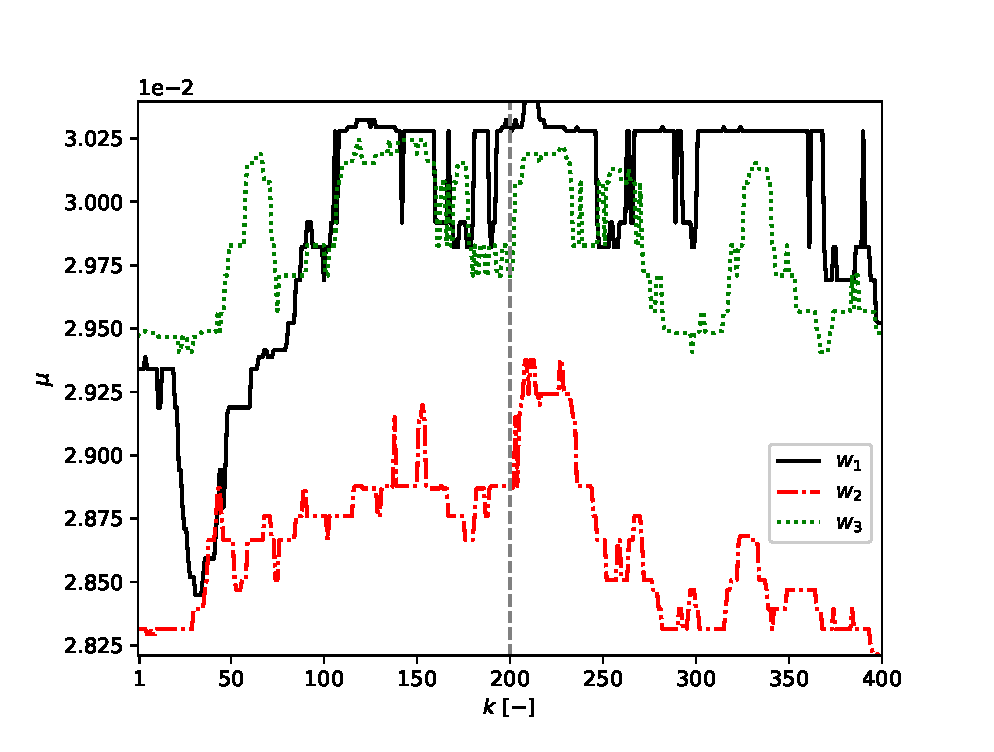
\includegraphics[scale=0.71]{IMG/appel_par/par_mu.eps}
	\caption{Hodnota parametru $\mu$ GPD pro všechny tři adaptivní váhy $w_1$, $w_2$, $w_3$ během experimentu detekce změn parametrů generátoru signálu. Svislá čára v diskrétním časovém okamžiku $k=200$ znázorňuje skokovou změnu parametrů generátoru signálu.}
		\label{fig:par_mu}
\end{figure}

\begin{figure}[h!]

	\centering
	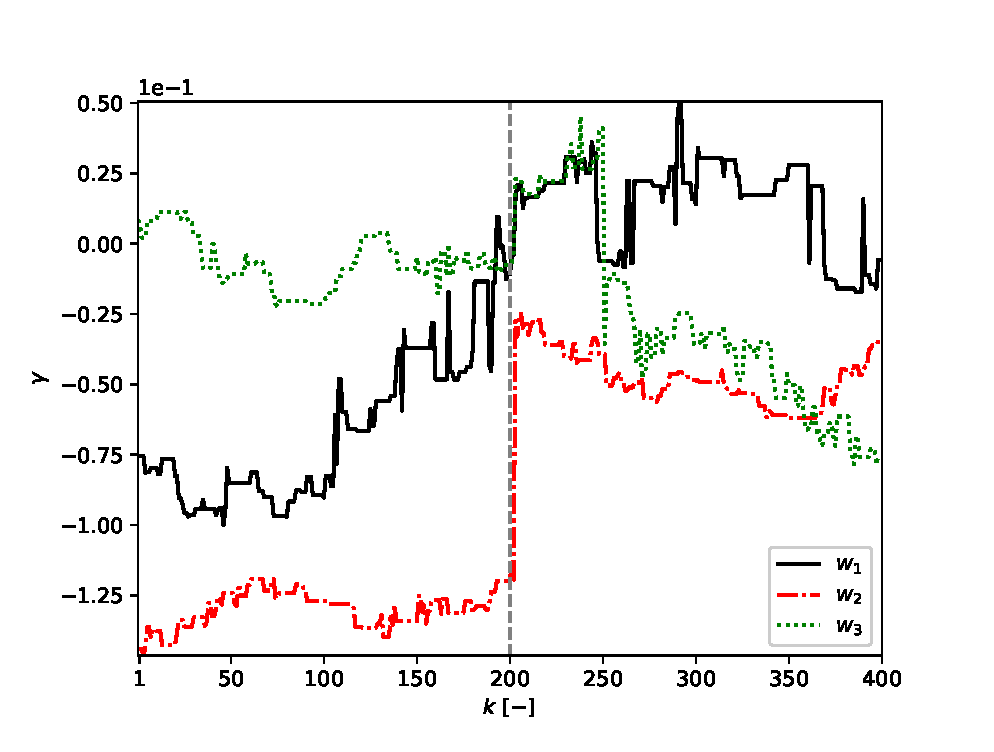
\includegraphics[scale=0.71]{IMG/appel_par/par_gamma.eps}
	\caption{Hodnota parametru $\gamma$ GPD pro všechny tři adaptivní váhy $w_1$, $w_2$, $w_3$ během experimentu detekce změn parametrů generátoru signálu. Svislá čára v diskrétním časovém okamžiku $k=200$ znázorňuje skokovou změnu parametrů generátoru signálu.}
		\label{fig:par_gamma}
\end{figure}

\begin{figure}[h!]

	\centering
	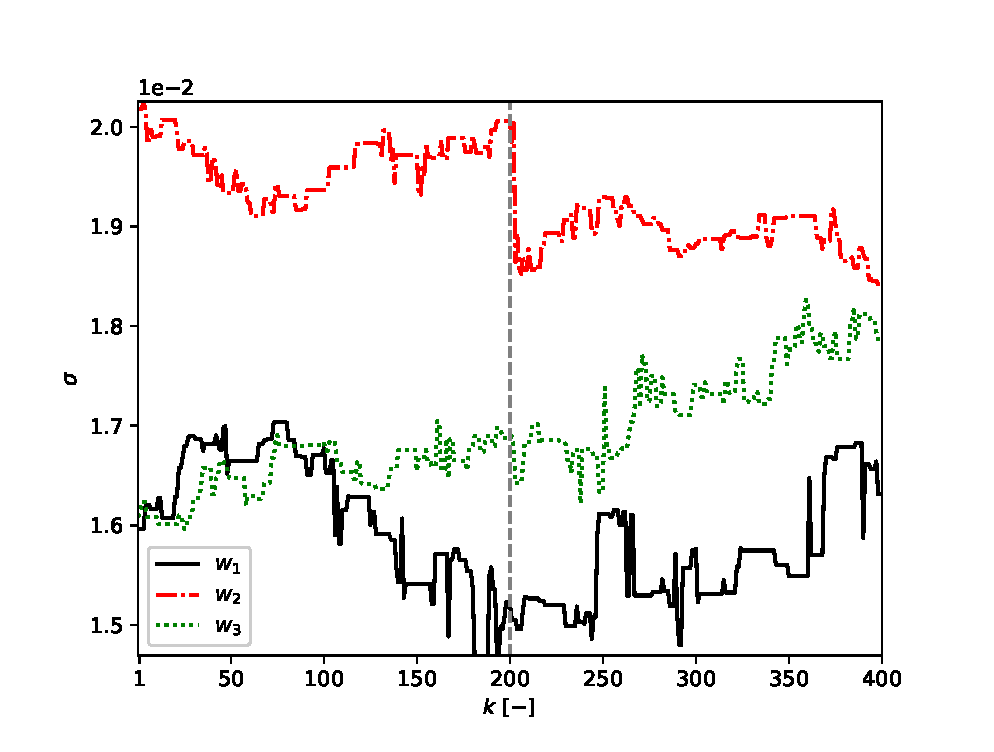
\includegraphics[scale=0.71]{IMG/appel_par/par_sigma.eps}
	\caption{Hodnota parametru $\sigma$ GPD pro všechny tři adaptivní váhy $w_1$, $w_2$, $w_3$ během experimentu detekce změn parametrů generátoru signálu. Svislá čára v diskrétním časovém okamžiku $k=200$ znázorňuje skokovou změnu parametrů generátoru signálu.}
		\label{fig:par_sigma}
\end{figure}
Průměrný čas výpočtu $\overline{t}$ parametrů všech tří GPD (počet GPD odpovídá počtu adaptivních parametrů filtru) a odpovídající směrodatné odchylky $\sigma_t$ jsou uvedeny v následující tabulce \ref{tab:par_results}. Čas výpočtu je určený pro jeden experiment (400 vzorků).
\begin{table}[h!]

\centering
\caption{Tabulka průměrných časů výpočtu pro jednotlivé adaptivní váhy a odpovídajících směrodatných odchylek vybraných metod výpočtu parametrů GPD}
\begin{tabular}{|l|l||l|l|}
\hline
 & Metoda & $\overline{t}$ {[}ms{]} & $\sigma_t$ {[}ms{]} \\ \hline \hline
\multirow{3}{*}{$w_1$} & ML & $26.198$ & $3.396$ \\ \cline{2-4} 
 & QML & $0.354$ & $0.478$ \\ \cline{2-4} 
 & MOM & $\textbf{0.076}$ & $0.264$ \\ \hline
\multirow{3}{*}{$w_2$} & ML & $26.718$ & $2.302$ \\ \cline{2-4} 
 & QML & $0.337$ & $0.471$ \\ \cline{2-4} 
 & MOM & $\textbf{0.064}$ & $0.244$ \\ \hline
\multirow{3}{*}{$w_3$} & ML & $24.982$ & $1.964$ \\ \cline{2-4} 
 & QML & $0.395$ & $0.489$ \\ \cline{2-4} 
 & MOM & $\textbf{0.060}$ & $0.238$ \\ \hline

\end{tabular}
 \label{tab:par_results}
\end{table}

Z uvedených výsledků je patrné, že nejrychlejší metoda je MOM. Podstatnou nevýhodou této metody pro využití v aplikacích, které vyhodnocují data v reálném čase je její omezení na hodnoty parametrů GPD (viz kapitola \ref{chap:gpd}). Pokud parametry uvedené omezení nesplňují, vypočtené hodnoty nepřesné (resp. nesmyslné) a tedy nepoužitelné pro algoritmus ESE, který začne produkovat nepřesné výsledky. Z pohledu úlohy detekce novosti je diskutabilní, zda-li můžeme garantovat, že sledovaný proces po celou dobu bude splňovat uvedené omezení.
\par
Metoda, jejíž výpočetní čas byl nejvyšší je ML, což je vzhledem k iterativnímu určení parametrů GPD očekávatelné. Nevýhoda použití této metody tkví v  nemožnosti určit minimální resp. maximální počet iterací. Jednou z možností jak zrychlit nalezení parametrů je využití apriorní informace o hodnotách těchto parametrů. V rámci experimentu však byla využita pouze apriorní informace o parametru $\mu$, který odpovídá nejmenší hodnotě přírůstku vah, které byli získány metodou POT aplikovanou na plovoucí okno délky $n_s$.
\par
Dobrým kompromisem mezi výše uvedenými metodami je použití metody QML. Výpočetní čas této metody byl v uvedeném experimentu o dva řády kratší než ML a asi pětkrát delší než MOM. Pro každou z vyhodnocovaných vah byl kratší než $500$ $\mu s$.
\par 
Z provedeného experimentu je patrné, že použití algoritmu ESE pro aplikace v reálném čase je limitováno počtem parametrů filtru a rychlostí vzorkování monitorovaného procesu. 







 